Mono-Z analyses use events with a reconstructed Z boson recoiling symmetrically against \MET to detect the production of invisible particles.
In previous LHC analyses~\cite{Aaboud:2017bja,Sirunyan:2017qfc}, the DM interpretations of the analysis results have focused on either invisible decays of the SM-like Higgs bosons or topologies where the Z boson is produced as initial-state radiation (ISR) off a quark. The ISR-based topologies generically favor radiation of a gluon or photon rather than a massive gauge boson, thus limiting the discovery sensitive of a Z-based approach compared to monojet and mono-photon searches. In contrast, the model studies in this document generates the mono-Z signature dominantly via the all-bosonic H-a-Z vertex, which can lead to enhancements of the mono-Z sensitivity compared to jet and photon signature. In this section, the behavior and experimental accessibility of the model in Z+\MET events is studied.

\paragraph{Technical setup}
Simulated event samples for the leptonic mono-Z signature are produced with Madgraph5\_aMC@NLO version 2.4.3, interfaced with Pythia version 8.2.2.6 for parton showering. The NNPDF3.0 PDF set is used at LO precision with the value of the strong coupling constant set to $\alpha_{S}(M_{Z}) = 0.130$ (NNPDF30\_lo\_as\_0130). A five floavor scheme with a massless b-quark is used.  Only contributions from gluon-gluon initial states and \lp\lm$\chi\overline{\chi}$ final states are considered, where l = e or $\mu$. No additional matrix element partons are considered and diagrams with an intermediate s-channel SM Higgs boson are explicitly rejected to increase the calculation efficiency (generate g g $>$ xd xd~ l+ l- / h1). 


\paragraph{Event selection}
Three consecutive stages of event selection are considered:
\begin{itemize}
\item Inclusive: Lepton \pt and $\eta$ requirements corresponding to the typical experimental trigger acceptance are applied.

\item Preselection: A dilepton candidate with an invariant mass in a window around the Z mass is required, and a minimum transverse momentum of the $\chi\overline{\chi}$ system is required.

\item Final selection: Requirements on the main variables used in the relevant analyses are added: The angular separation in the transverse plane between the $\chi\overline{\chi}$ and \lp\lm systems $\Delta\Phi(ll,\MET)$, the relative transverse momentum difference between them $|p_{T,ll} - \MET|/p_{T,ll}$ and the angular separation between the leptons $\Delta R(ll)$. Additionally, the \MET requirement is tightened.
\end{itemize}

The exact event selection criteria are listed in Tab.~\ref{tab:monozll_selection}.

\begin{table}
\centering
\caption{Event selection requirements for the analysis of the Mono-Z signature with leptonic Z decays.
        The requirements are inspired to follow those used in typical experimental analyses.}
\begin{tabular}{c | c |r l}
Selection stage & Quantity & Requirement \\\hline


\multirow{ 2}{*}{Inclusive}         & lepton $\left|\eta\right|$                    & $< 2.5$ \\
                                    & leading (trailing) lepton \pt                 & $> 25 (20)$ GeV \\\hline

\multirow{ 2}{*}{Preselection}      & $\left|m_{ll}-m_{Z,\mathrm{nominal}}\right|$  & $< 15$ GeV\\
                                    & \MET                                          & $> 40$ GeV \\\hline

\multirow{ 3}{*}{Final selection}   & $\Delta\Phi(ll,\MET)$                         & $>2.7$\\
                                    &$|p_{T,ll} - \MET|/p_{T,ll}$                   & $<0.4$\\
                                    &  $\Delta R(ll)$                               & $<1.8$\\
\end{tabular}


\label{tab:monozll_selection}

\end{table}


\paragraph{Cross-sections, kinematic distributions and acceptance}
The overall cross-sections in the \tanb and mass scans are shown in Fig.~\ref{fig:monoz_ll_xs_inclusive}.
In the mass scan, maximal cross-sections are observed for the region of $\ma < \mA$ for values of $\ma\gtrsim100$ GeV. Towards higher values of both \ma and \mA, the cross-sections fall off, reaching values smaller than $1$ fb at $\ma\approx450$ GeV or $\mA\approx1.1$ TeV. In the $\ma\approx\mA$-region, the cross-section is suppressed by destructive interference. For the region with inverted mass hierarchy $\ma>\mA$, cross-sections of the order of multiple fb are observed, as long as $|\ma-\mA|$ remains sufficiently large.
In the \tanb scan, cross-sections smoothly fall with increasing $\ma$ as well as $\tanb$. Cross-sections are typically larger than 1 fb up to $\tanb\approx5$. The dependence on $\ma$ is modulated by the value of \tanb: Crossing the $\ma$ range from $100$ to $400$ GeV, cross-sections are reduced by a factor $\approx7$ for small $\tanb\approx1$, but only a factor $\approx2$ for higher values of $\tanb\approx5$.
For the \sinp scan shown in Figure \ref{fig:monoz_ll_sinp_scan_xsec}, the \sinp impact depends on whether or not the $a \rightarrow \ttbar$ decays are accesible.  
For \ma < 350 GeV they are not accesible and cross section strictly increases with \sinp.  For \ma > 350 \GeV, the $a \rightarrow \ttbar$ decays become possible causing the cross section to decrease for large values of \sinp.

%For \ma <350 GeV they are not accesible,  and only the heavy scalar's branching fraction to $aZ$ is relevant.  This branching fraction stricly increases with \sinp.  For \ma > 350 \GeV, the branching fraction of $a \rightarrow \chi \chi$ also becomes important, and there is a turnover point were the cross section decreases.


Acceptances for the mass and \tanb scans are shown in Figures \ref{fig:monoz_ll_acceptance} and \ref{fig:monoz_ll_tanbma_acceptance}.  
In the mass scan, for points where the Jacobian Peak is below the analysis's \MET cut, from $\ma = 100$ $\mA = 200$ to $\ma = 300$ $\mA = 400$, 
acceptance drops sharply approaching zero.  Above this region, acceptance curves are grouped into bands for fixed values of $\mA-\ma$.  
Acceptances increase with increasing $\mA-\ma$, gradually plateauing to a maximum value of 50\%.  In the inverted mass region, 
acceptance is generally lower than the rest of the mass scan, but for light values of \ma can reach values as large as 30\%.
In the \tanb scan, acceptance is largely independent of \tanb and constant for equal values of \ma.

To assess the kinematic behavior of the signal, the distributions of the kinematic variables that are most relevant to the Mono-Z signature are studied as a function of the model parameters.

Similar to mono-h, in the mono-Z channel a resonantly produced heavy scalar, $H$, decaying to $aZ$ produces a characteristic Jacobian peak in the \MET distribution.  The location of this peak depends on \mH, \ma, and $M_{Z}$ as given by equation \ref{eq:monoz_jacobian_peak}.  Figure \ref{fig:monoz_ll_mA_scan} shows how the position of the Jacobian peak shifts for increasing values of \mH.  For this paper, a subset of models are studied where \mA is degenerate with \mH.    

\begin{align}
E^{\mathrm{miss},max}_T \approx \frac{\sqrt{\left(\mH^2 -\ma^2 -M_{Z}^2\right)^2 - 4 \ma^2 M_{h}^2}}{2\mZ}\,.
\label{eq:monoZ_jacobian_peak}
\end{align}

The distribution of the invariant masses of the dilepton and $\chi\chi$ systems are shown in Fig.~\ref{fig:monoz_kin_inclusive}. Independent of the parameters, the dilepton mass spectrum is centered at the Z peak, without any nonresonant contribution. The $M_{\chi\chi}$ distribution illustrates the signal contributions from different diagrams. For $\mA>\ma$, DM is dominantly produced from on-shell $a$ boson production. In the inverted mass region $\mA<\ma$, the situation is reversed, and $H$ diagrams dominate.

After applying the preselection requirements, the distributions of kinematic variables are shown in Fig.~\ref{fig:monoz_kin_presel}. In the region of $\mA>\ma$, distinct Jacobian peaks are visible in the distributions of the mediator \pt, the width of which generally increases with values of $\ma$ and $\mA$. Significant portions of the spectrum are situated at relatively high boosts ($\MET>\unit[200]{GeV}$), which is more easily accessible experimentally.
This behavior is contrasted by the distributions in the inverted mass regions, which show nearly no distinct features and are mainly located at low mediator \
pt. For $\mA\approx\ma+m_{Z}$, both the a and Z bosons are produced approximately at rest, leading to an event population with overall low boost. These qualitative trends are consistent between the observables studied here.

Finally, the distributions of the $\MET$ and $\MT$ variables after final selection are shown in Fig.~\ref{fig:monoz_kin_final}. Traditionally, the Mono-Z search has relied on the $\MET$ distribution for signal extraction. While the presence of the Jacobian peak structure in the distribution facilitates signal-background separation, it may be beneficial to also consider the $\MT$ distribution. Although only transverse information is available, the resonant structure of the signal is significantly enhanced in the $\MT$ variable, which may enhance the sensitivity of a specialized search strategy.

The \tanb and \sinp variables have minimal effect on the distributions of kinematic variables (Fig.~\ref{fig:monoz_kin_tanb_sintheta}).  For small values of $\tanb$ there is a slight softening and broadening of the \MET distribution due to the increased contribution from non-resonant $z+a$ production.


\paragraph{Expected significance}

Expected sensitivity for the Mono-Z(ll) channel to 2HDM+a models are approximated using generator level signal samples and published background estimates from recent $Z(\ell \ell) + \MET$ searches of 36.1 \ifb of data \cite{Aaboud:2017bja}.

Following the Asimov approximation, expected significance is calculated as the ratio of likelihoods given by equation \ref{eq:significance} and is valid even for $s$ not $\ll b$ \cite{Cowan:2010js}.  
This equation is modified to account for systematic uncertainties on the background (\ref{eq:significance_wsyst}) \cite{Cowan:2012}, and the total significance is taken as the per bin significances summed in quadrature.

For the signal events a reconstruction efficiency of 75\% is assumed.  To be consistent with the background estimates, the same selection cuts as \cite{Aaboud:2017bja} are used.  Signal and background are binned in \MET, and a conservative 20\% systematic on the background is assumed for \MET < 120 \GeV and 10\% above.

Expected significances are shown in Figure \ref{fig:expected_significance_monozll}, with regions the ATLAS and CMS detectors should be sensitive to, greater than 2, highlighted.

\begin{equation}
\label{eq:significance}
Z = \sqrt{2 \bigg( (s+b) \ln{1 + \frac{s}{b}} - S \bigg) }
\end{equation}


\begin{equation}
\label{eq:significance_wsyst}
Z^\prime_{bin} = \sqrt{ 2 \cdot \bigg( (s+b) \ln[\frac{ (s+b) (b+\sigma_b^2) } {b^2 + (s+b) \sigma_b^2} ]- \frac{b^2}{\sigma_b^2} \ln[1 + \frac{\sigma_b^2 s}{b(b+\sigma_b^2)} ] \bigg) }
\end{equation}

\begin{equation}
\mathcal{S} = \sqrt{\sum_{bin} (Z^\prime_{bin})^2}
\end{equation}

\paragraph{Conclusions} The Mono-Z(ll) provides experimental coverage of the pseudoscalar 2HDM model for a broad part of the parameter space. The light pseudoscalar \a can be probed up to mass values of $\approx\unit[350]{GeV}$, depending on the choice of other parameters. The Mono-Z is sensitive mostly in the region of low values of $\tanb<4$.

\begin{figure}
\centering
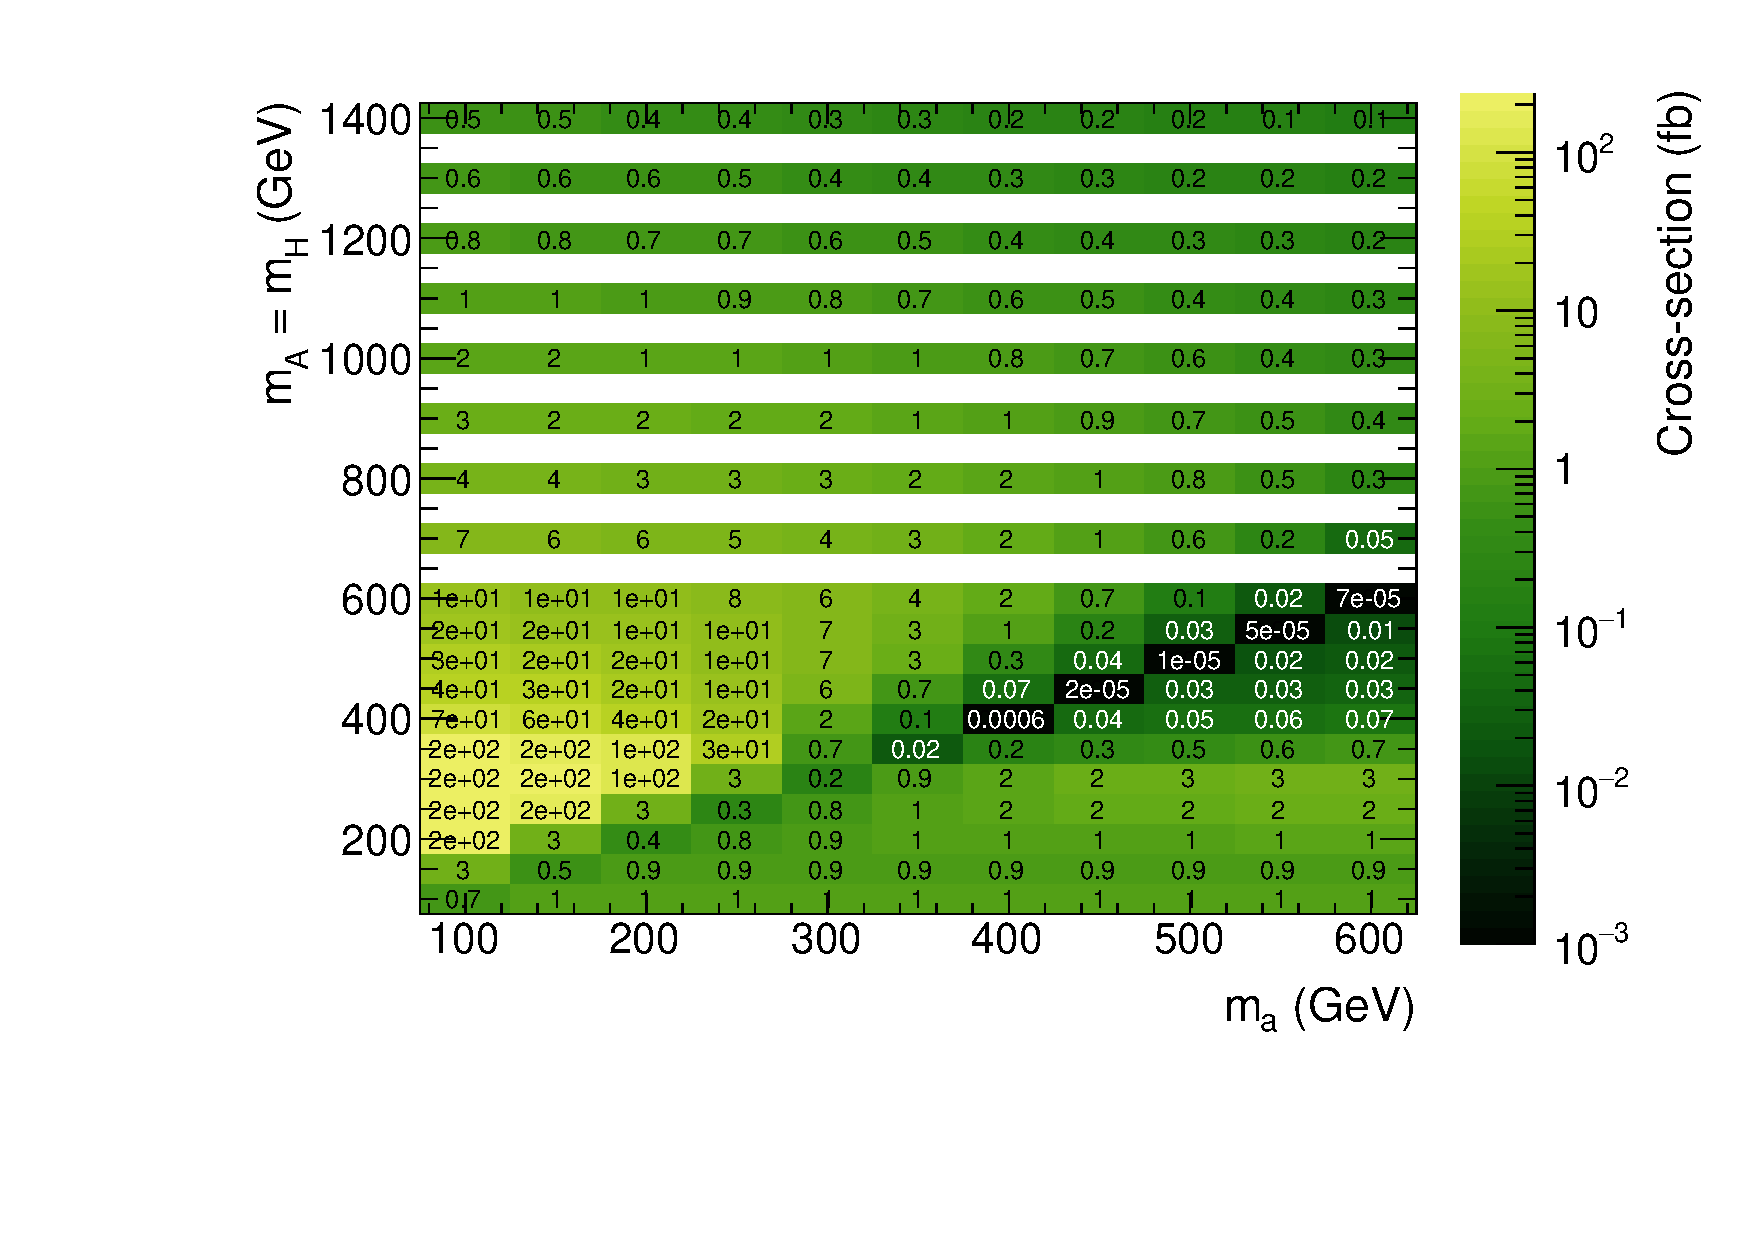
\includegraphics[width=0.8\textwidth]{texinputs/04_grid/figures/monoz/leptonic/xs_2d_inclusive_26300.pdf}
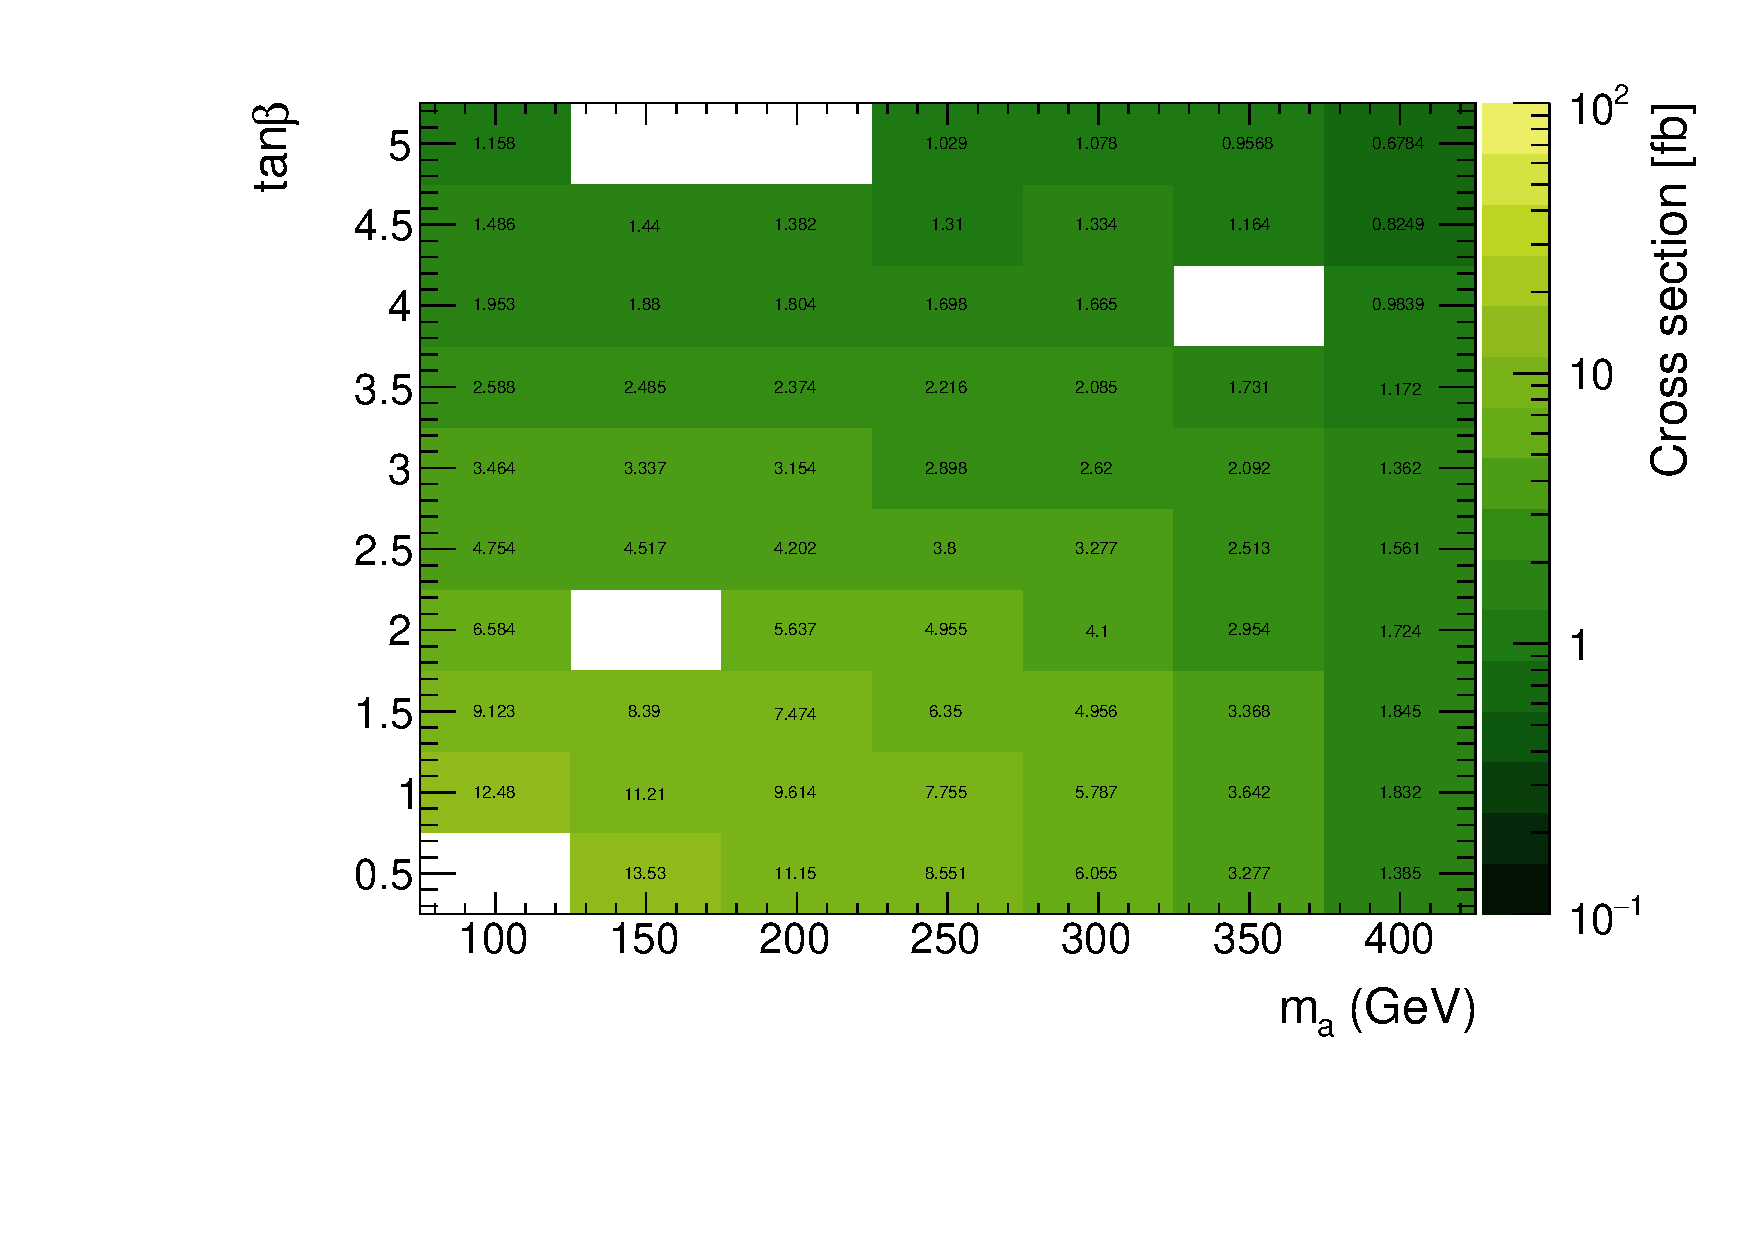
\includegraphics[width=0.8\textwidth]{texinputs/04_grid/figures/monoz/leptonic/tanbma_xsec_ll.pdf}
\caption{Inclusive cross-sections for $pp\rightarrow \lp\lm\chi\overline{\chi}$ in the \ma-\mA (top) and \ma-\tanb scans (bottom).}
\label{fig:monoz_ll_xs_inclusive}
\end{figure}


\begin{figure}
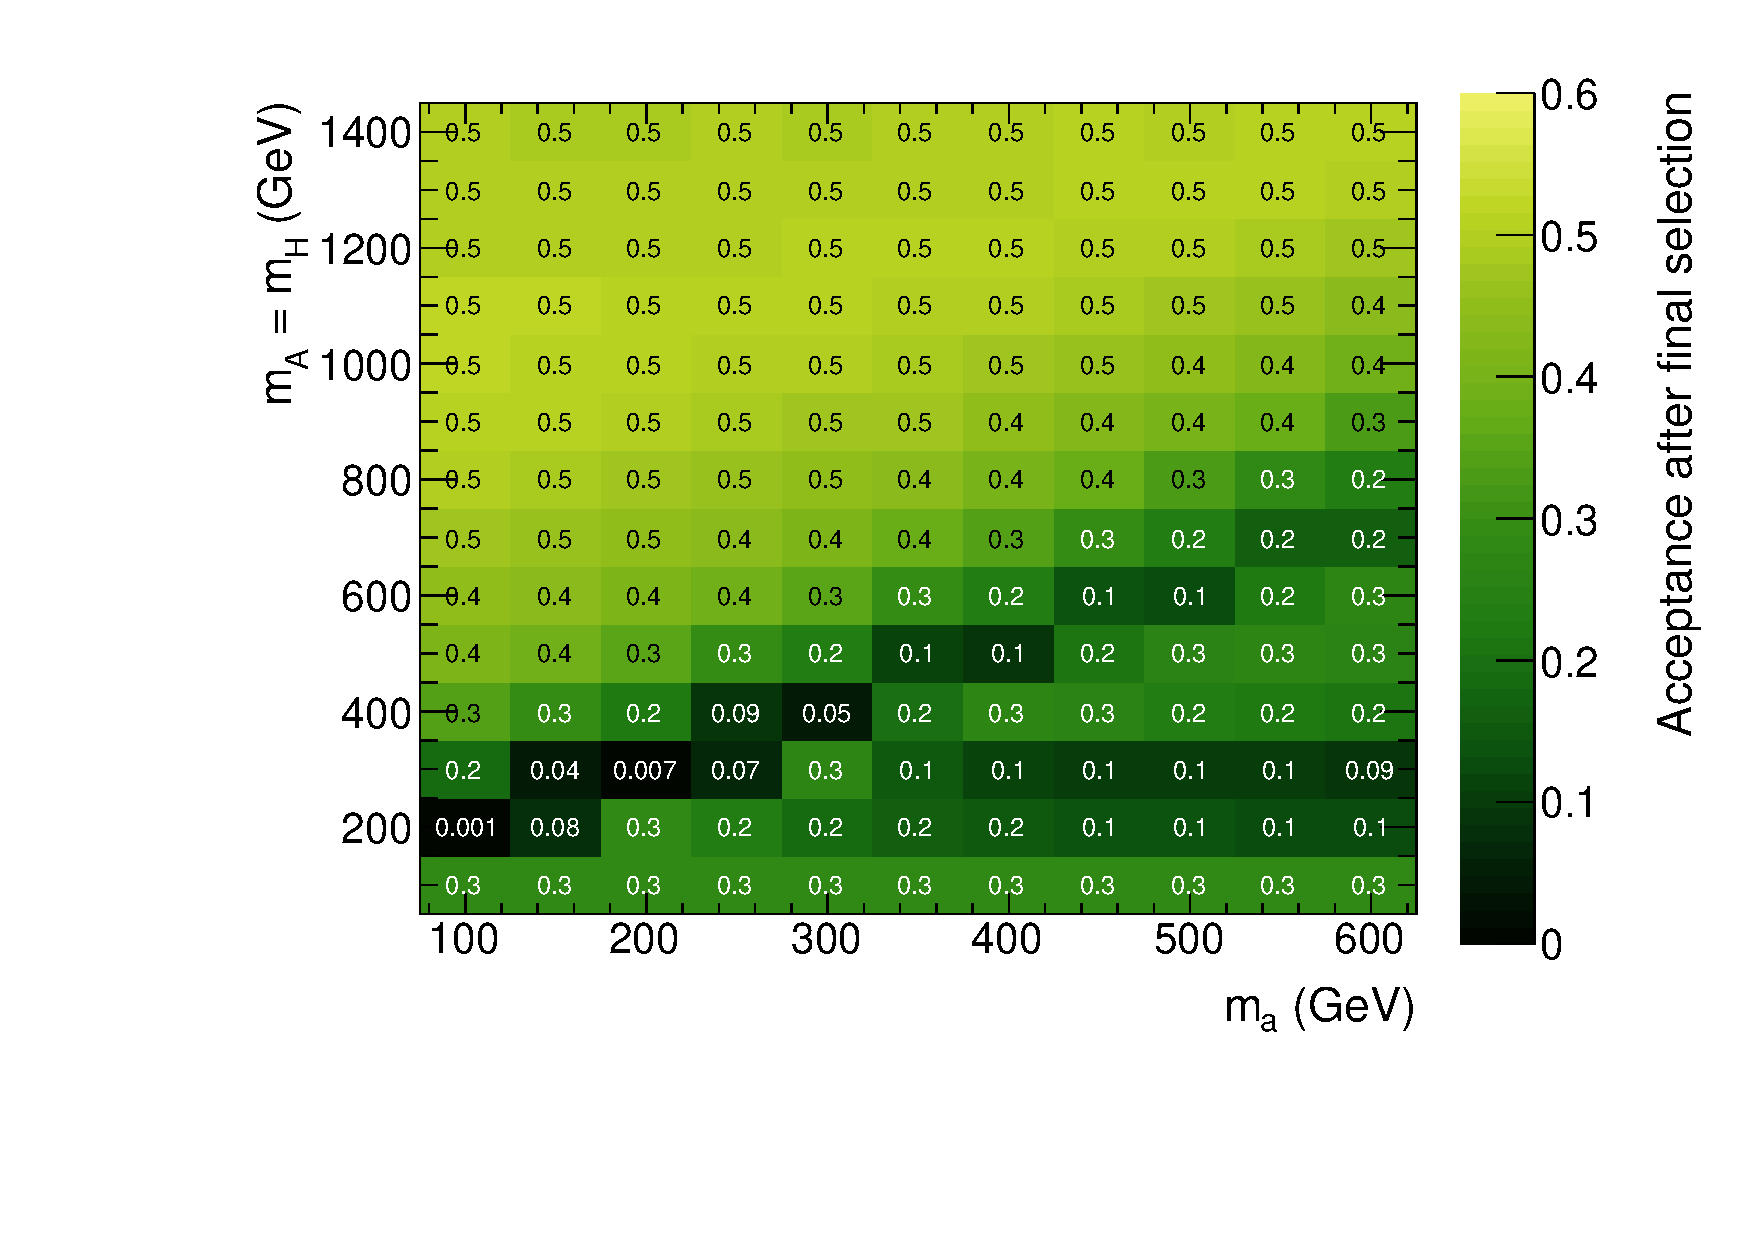
\includegraphics[width=\textwidth]{texinputs/04_grid/figures/monoz/leptonic/acceptance_dmwg-final_26300.pdf}
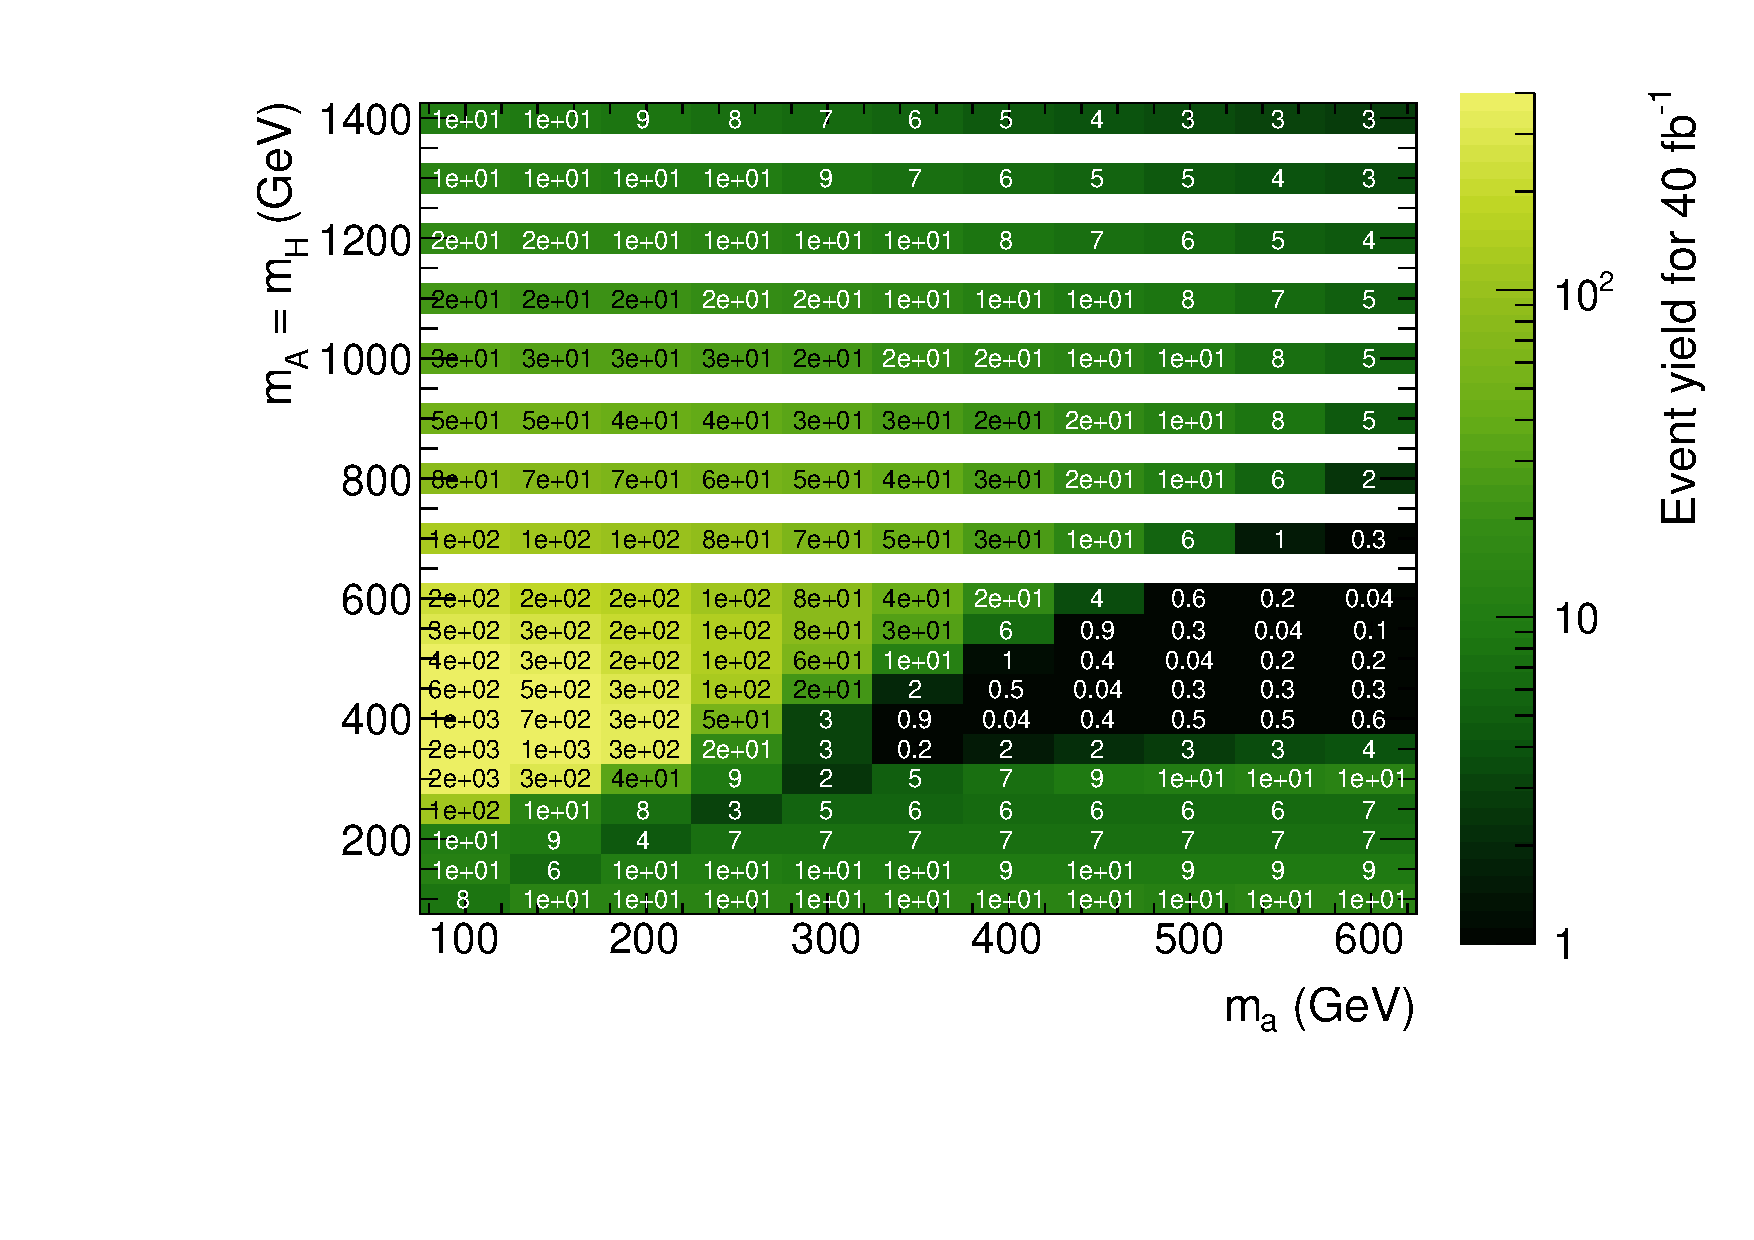
\includegraphics[width=\textwidth]{texinputs/04_grid/figures/monoz/leptonic/xs_2d_dmwg-final_26300_yield40fb.pdf}
\caption{Acceptance and event yields in the  \ma-\mA plane after applying the final selection. Event yields assume an integrated luminosity of $40~\ifb$. The acceptance is maximal for $\mA > \ma$, where it reaches 50 \%. In the inverted mass region $\mA < \ma$, lower values of 10-30\% are observed. In the intermediate region around $\mA \approx \ma + \mZ$, the acceptance is strongly suppressed as the a and Z bosons are produced approximately at rest.}
\label{fig:monoz_ll_acceptance}
\end{figure}

\begin{figure}
\centering
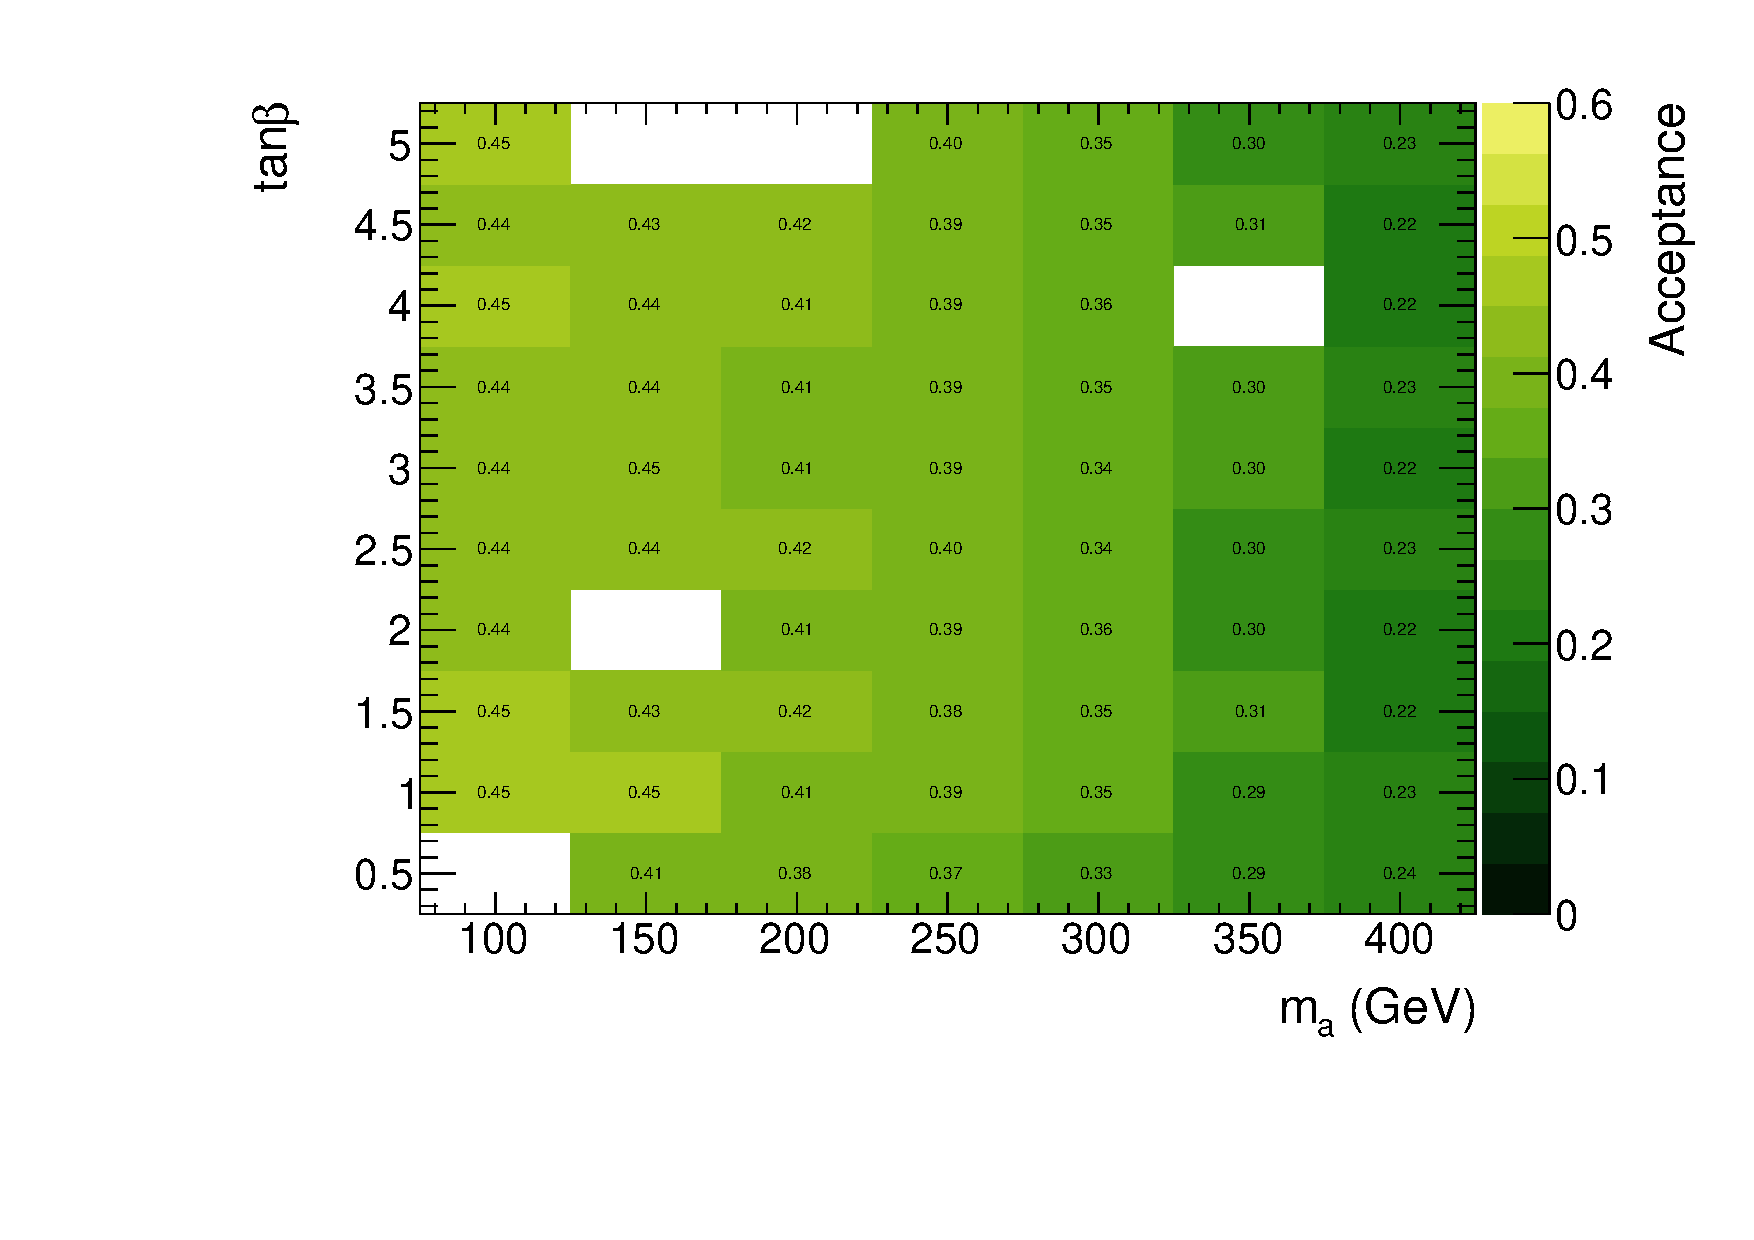
\includegraphics[width=0.9\textwidth]{texinputs/04_grid/figures/monoz/leptonic/tanbma_ae_ll.pdf}
\caption{Acceptances across the \ma-\tanb scan.  Acceptance is flat over \tanb for constant values of \ma.}
\label{fig:monoz_ll_tanbma_acceptance}
\end{figure}

\begin{figure}
\centering
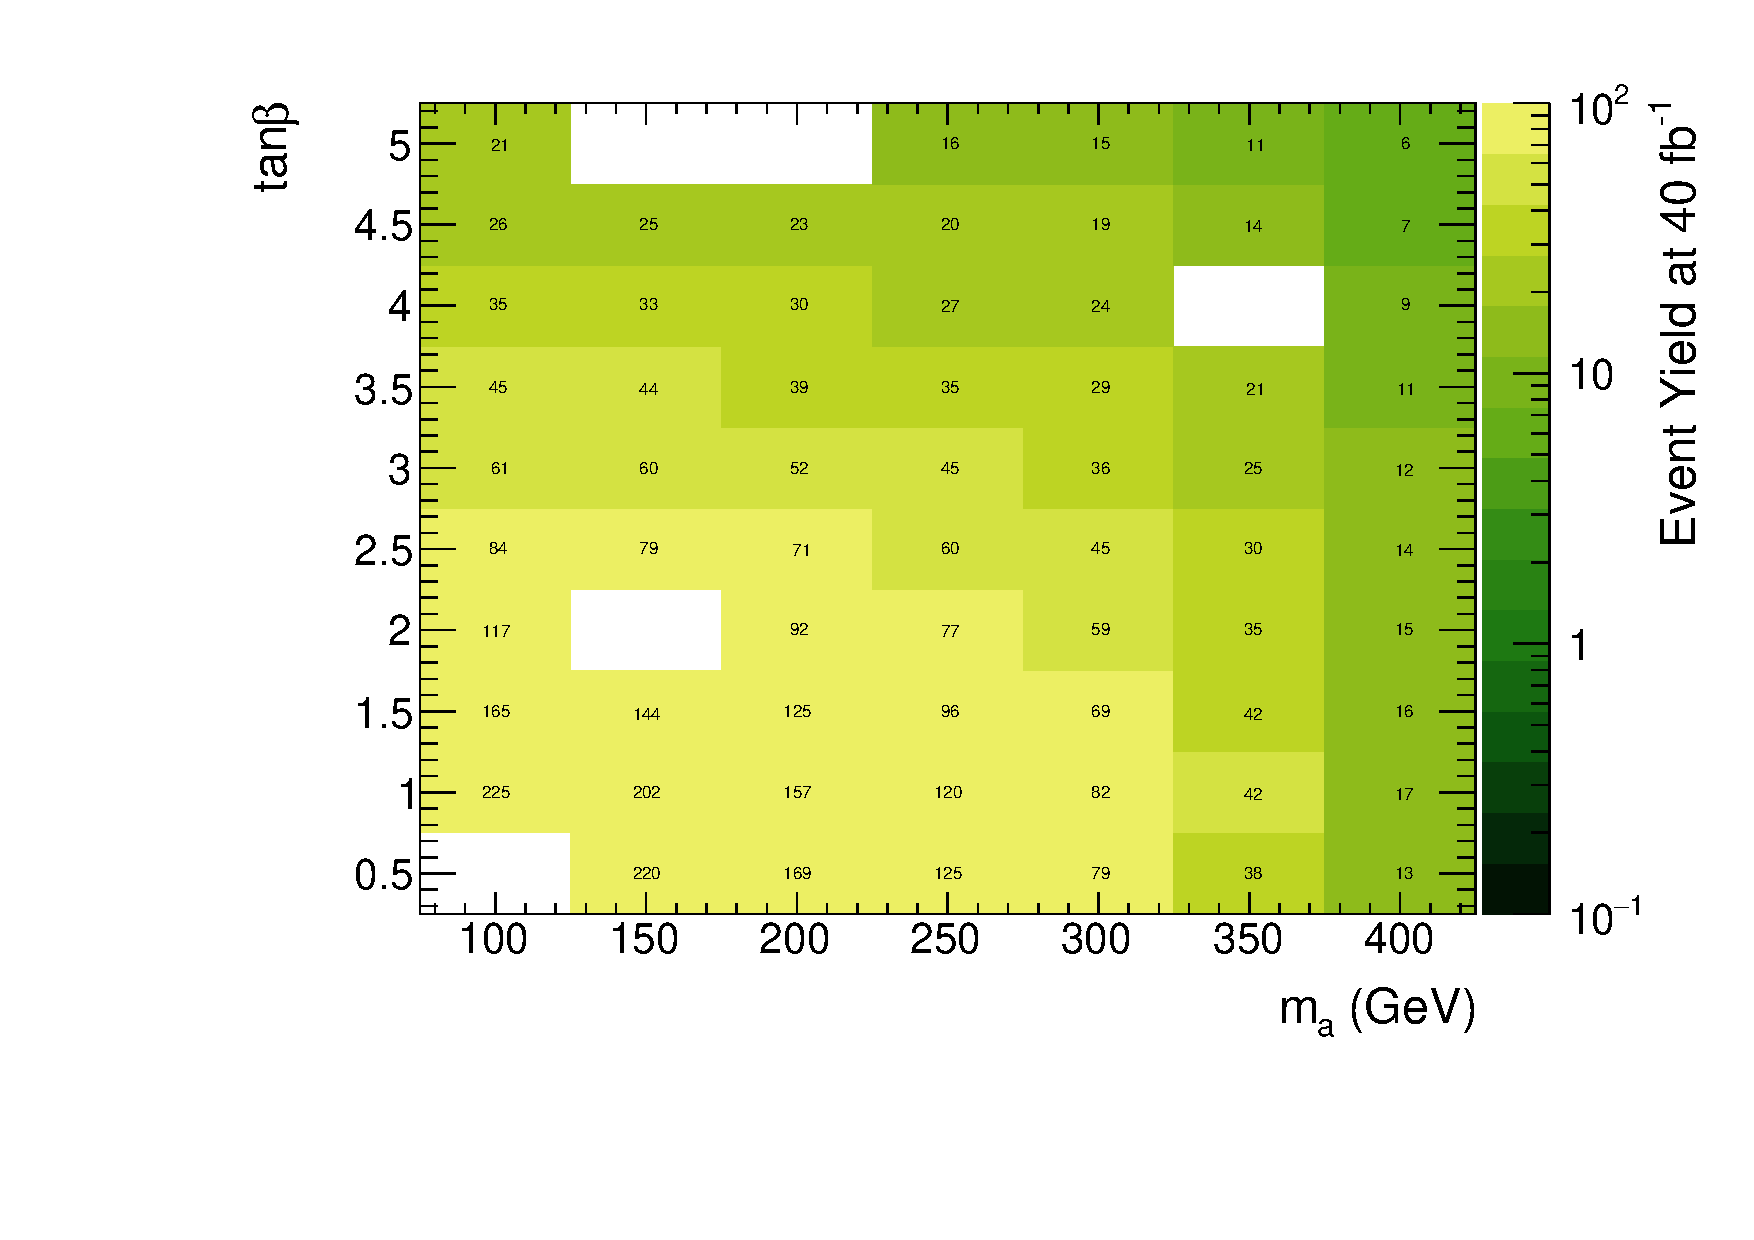
\includegraphics[width=0.9\textwidth]{texinputs/04_grid/figures/monoz/leptonic/tanbma_yield_ll.pdf}
\caption{Event yield in the \ma-tanBeta grid, for an integrated luminosity of $40~\ifb$.  The number of expected events diminshes with increasing tanBeta and \ma.  \mA fixed to 600 GeV and sinTheta to 0.35}
\end{figure}


\begin{figure}
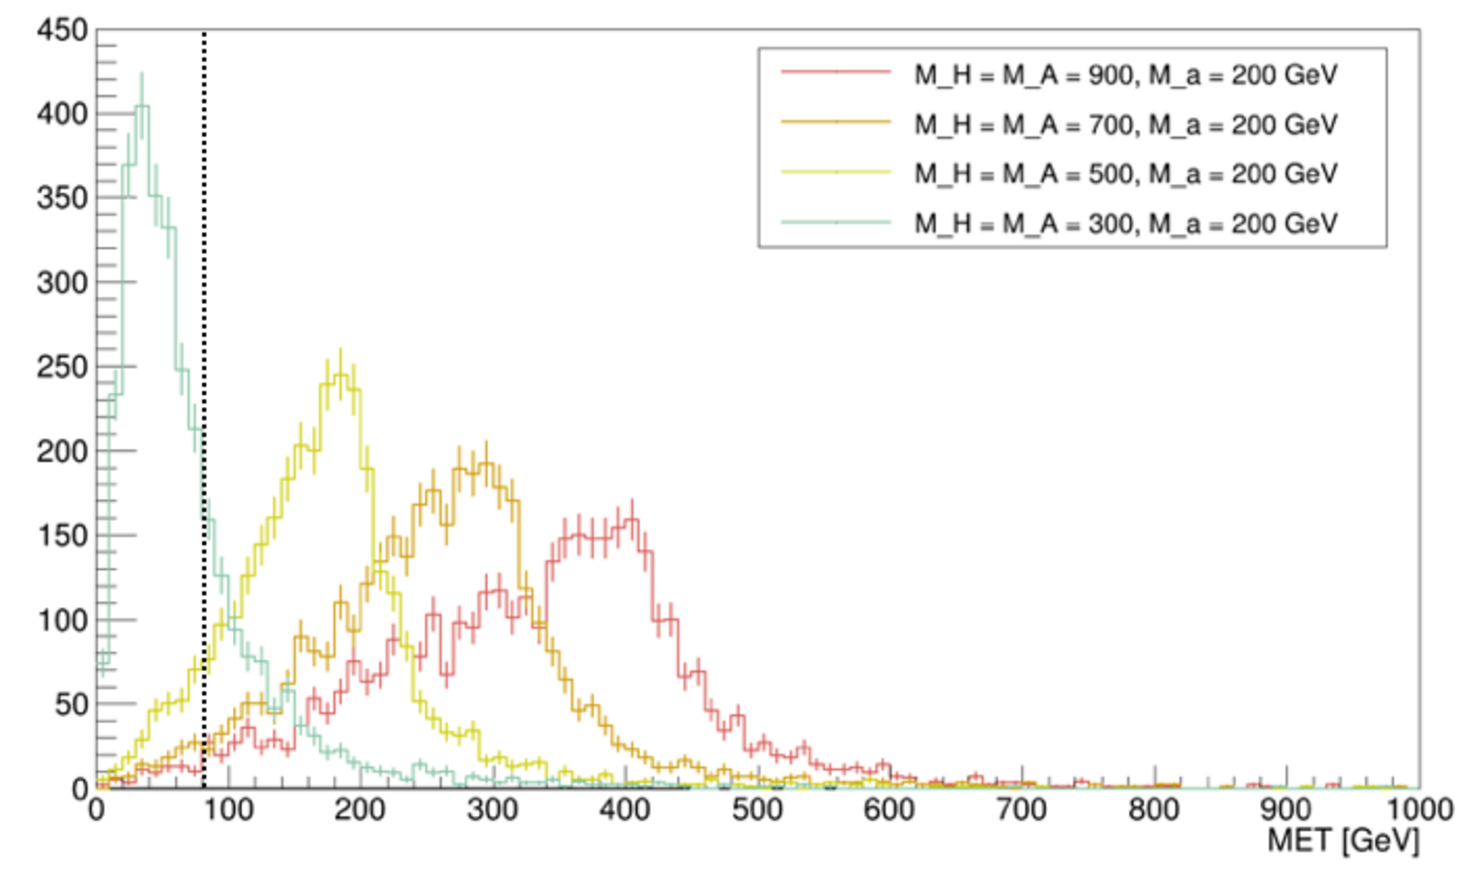
\includegraphics[width=0.9\textwidth]{texinputs/04_grid/figures/monoz/leptonic/mA_Scan.pdf}
\caption{The position of the Jacobian peak in the \MET distribution depends on the values of \mH, \ma, and $M_{Z}$.  This figure shows a scan of \mH values for fixed \ma and \mA = \mH.  Increasing the difference between \mH and \ma shifts the location of the peak towards high energies, whereas for small mass splittings the \MET distribution is soft and most events will fail to pass the \MET selection criteria.}   
\label{fig:monoz_ll_mA_scan}
\end{figure}

\begin{figure}
\centering
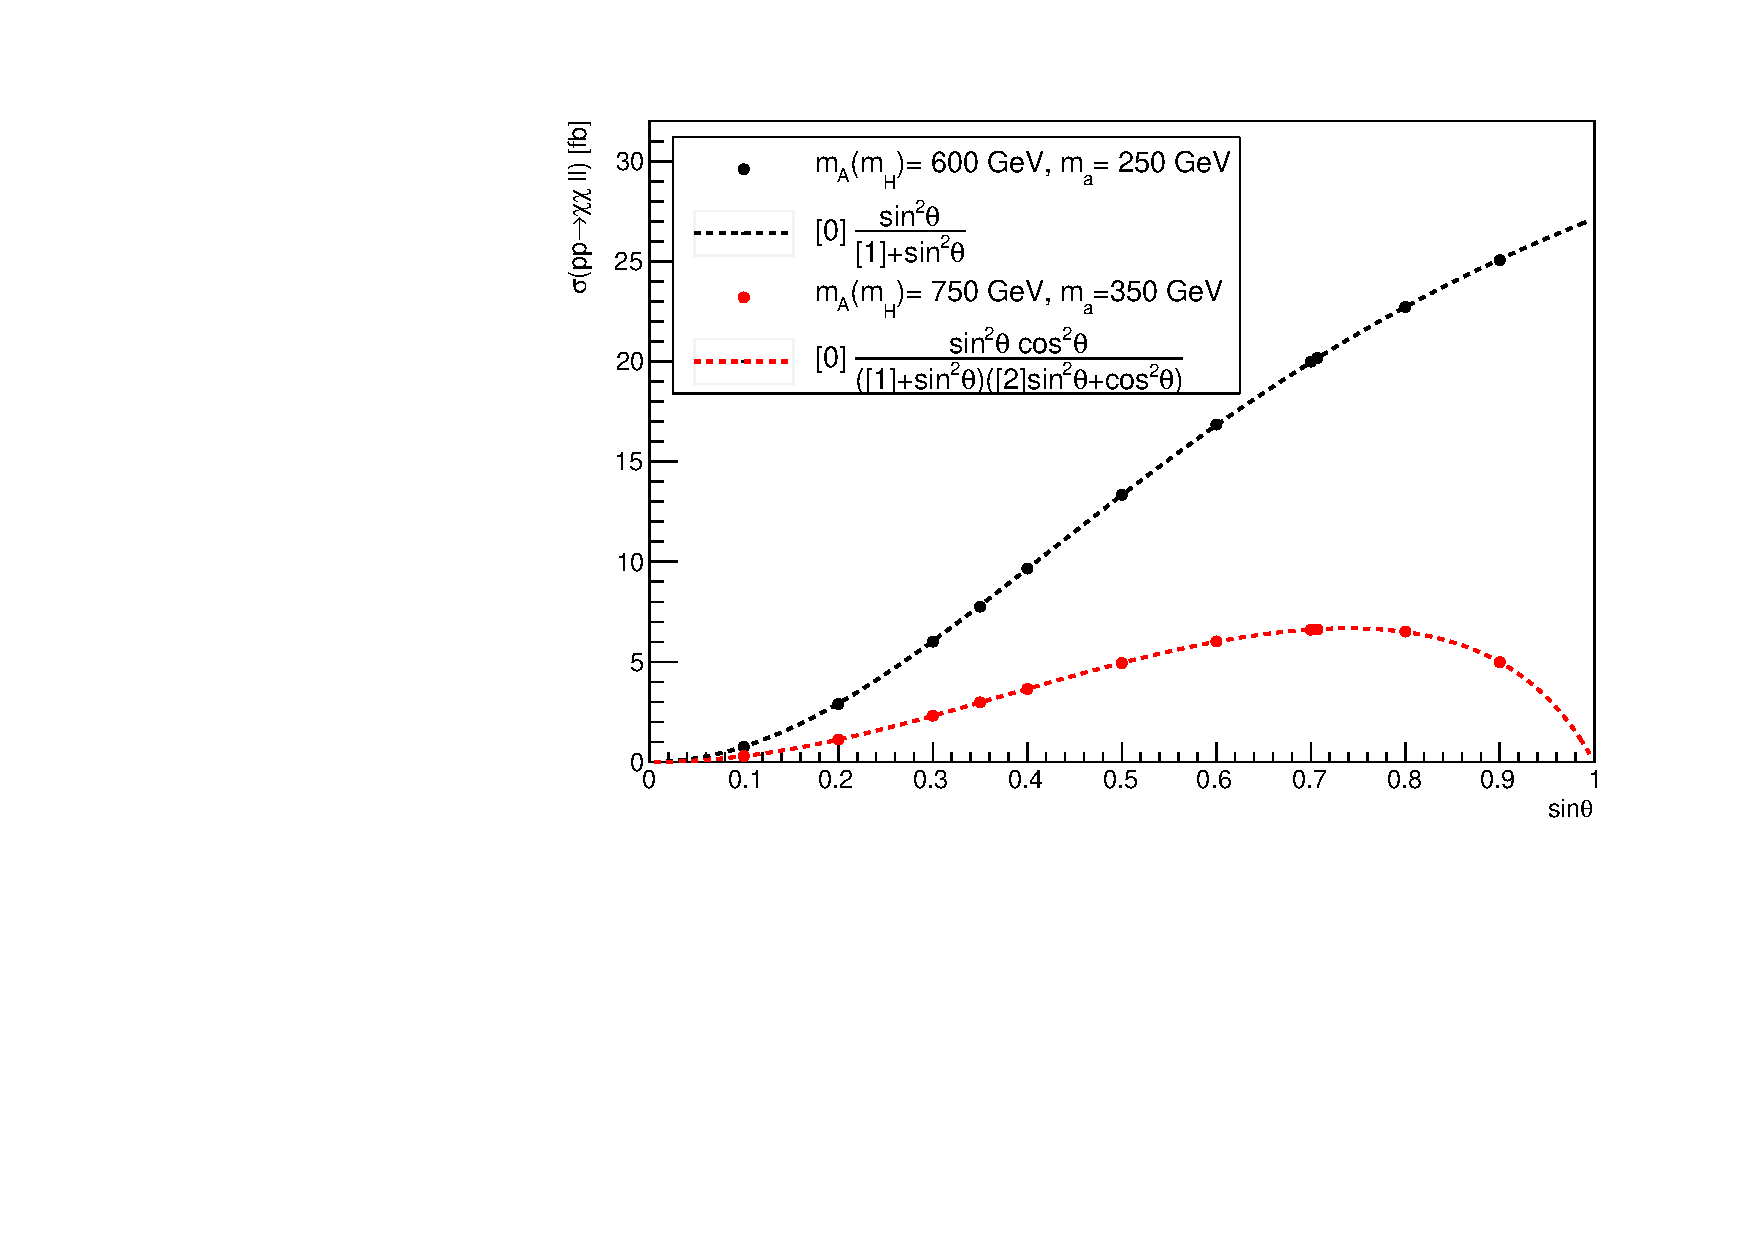
\includegraphics[width=0.6\textwidth]{texinputs/04_grid/figures/monoz/leptonic/SinThetaScan_xsecs.pdf}
\caption{For two different mass points, this figure shows the cross section $pp\rightarrow\chi\chi\ell\ell$ as a function of \sinp. 
For $\ma < 350$ GeV, $a$ decays solely to dark matter particles.  
As a consequence, the mixing angle only impacts the heavy scalar's branching fraction to $aZ$ and 
cross section strictly increases with \sinp.  
For \ma above 350 \GeV, \ttbar~ decays become accesible, introducing additional \sinp and \cosp dependences for the branching fraction 
of $a\rightarrow\chi\chi$.  For \ma above 350 GeV for large values of \sinp, there is a turnover point where the reduced $a\rightarrow\chi\chi$ branching fraction outweights the increased $H \rightarrow aZ$ branching and the net cross section decreases.}
\label{fig:monoz_ll_sinp_scan_xsec}
\end{figure}


\begin{figure}
\centering
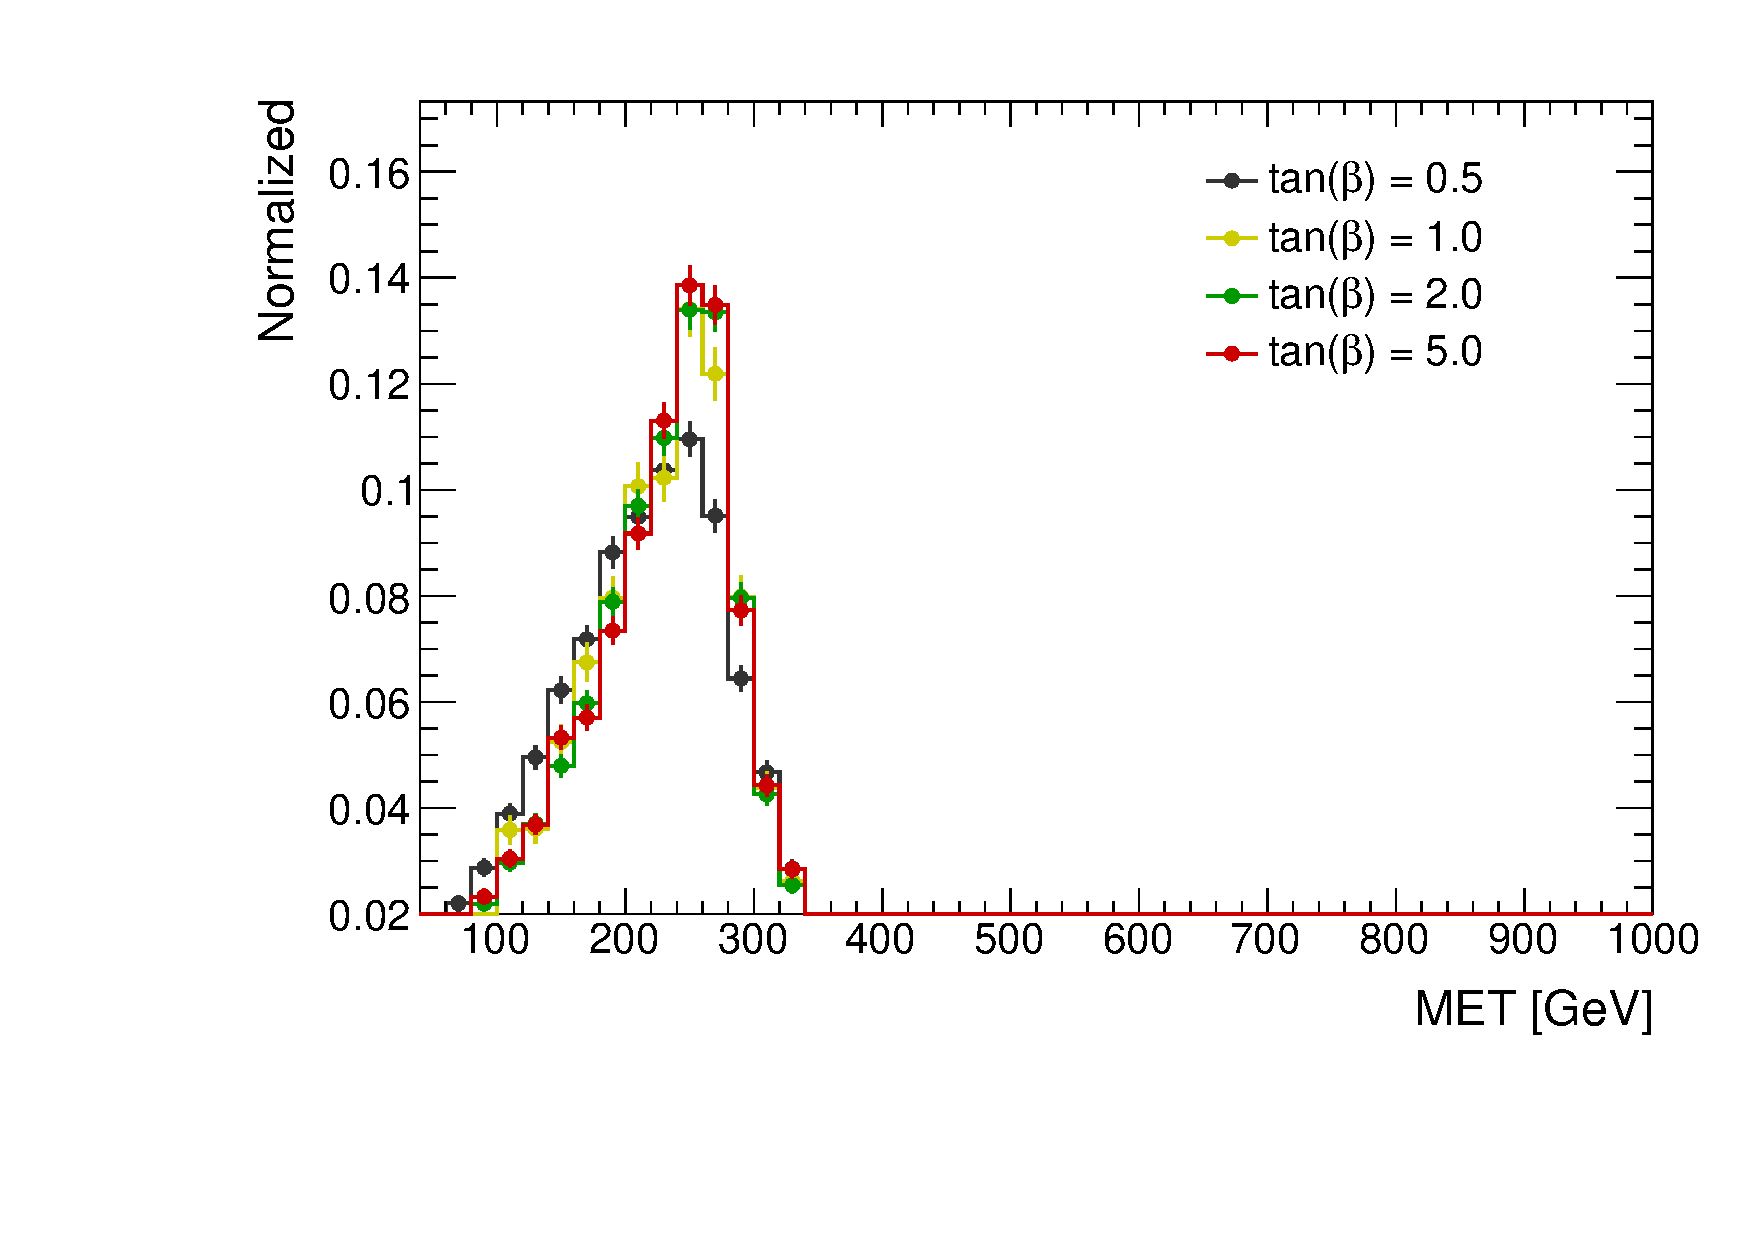
\includegraphics[width=0.45\textwidth]{texinputs/04_grid/figures/monoz/leptonic/TanbScan_mH600ma150_MET.pdf} 
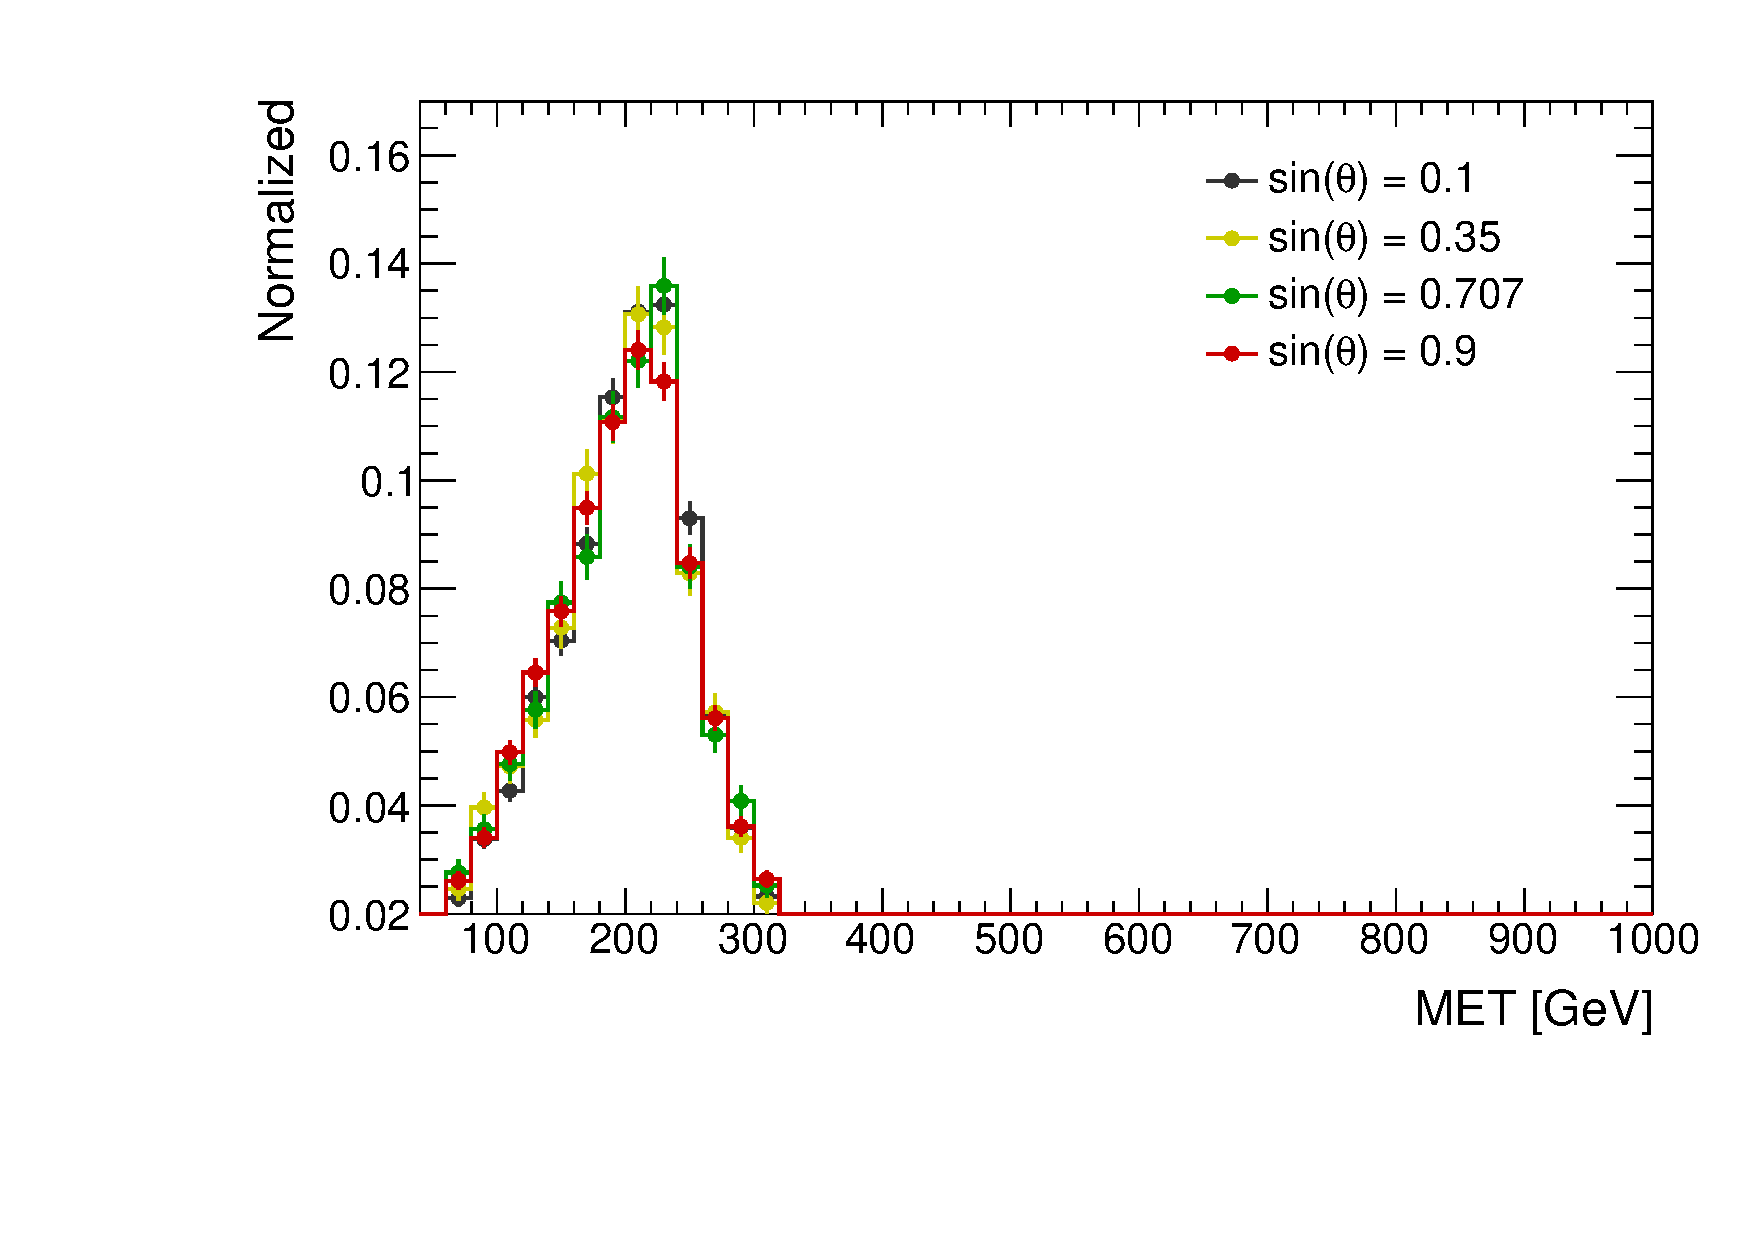
\includegraphics[width=0.45\textwidth]{texinputs/04_grid/figures/monoz/leptonic/SinpScan_mH600ma250_MET.pdf} 
%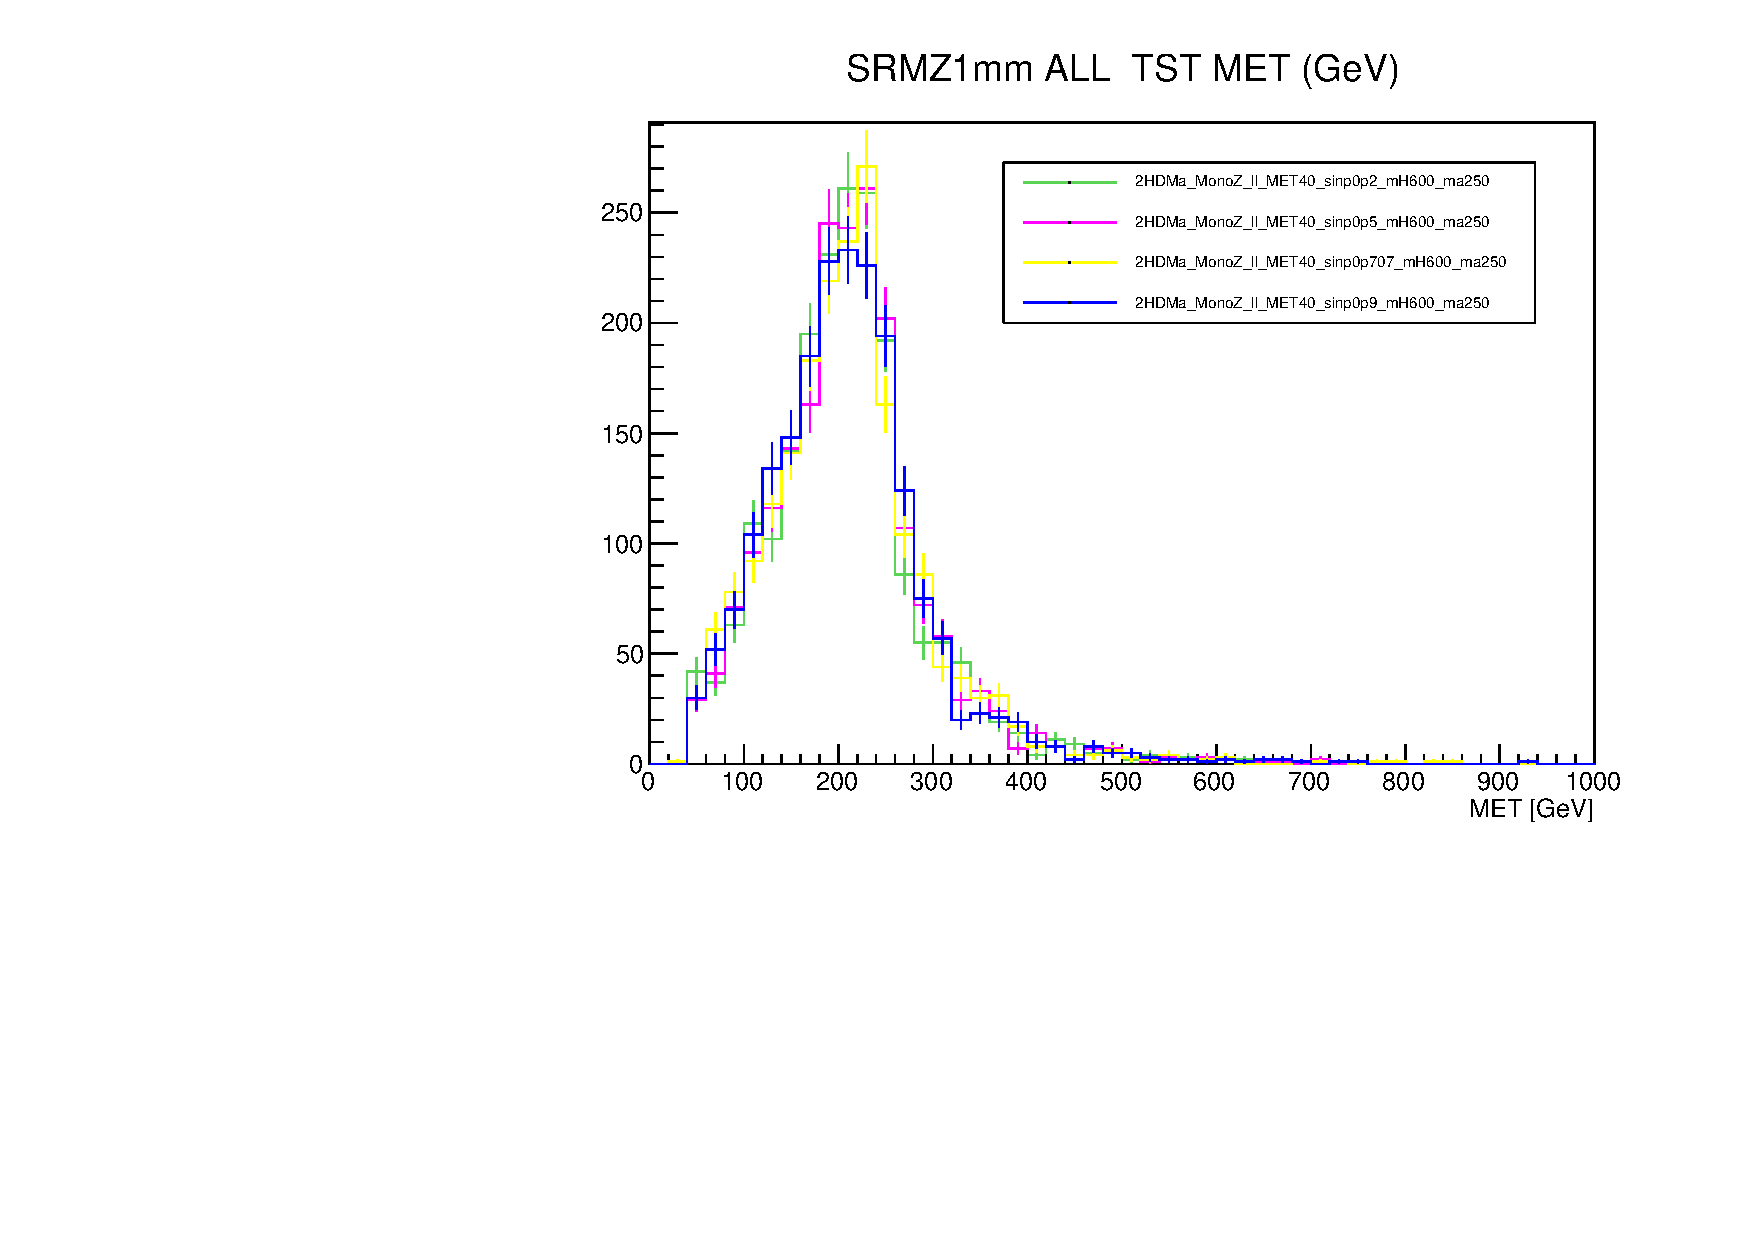
\includegraphics[width=0.45\textwidth]{texinputs/04_grid/figures/monoz/leptonic/SinThetaScan_mH600ma250_MET.pdf}
%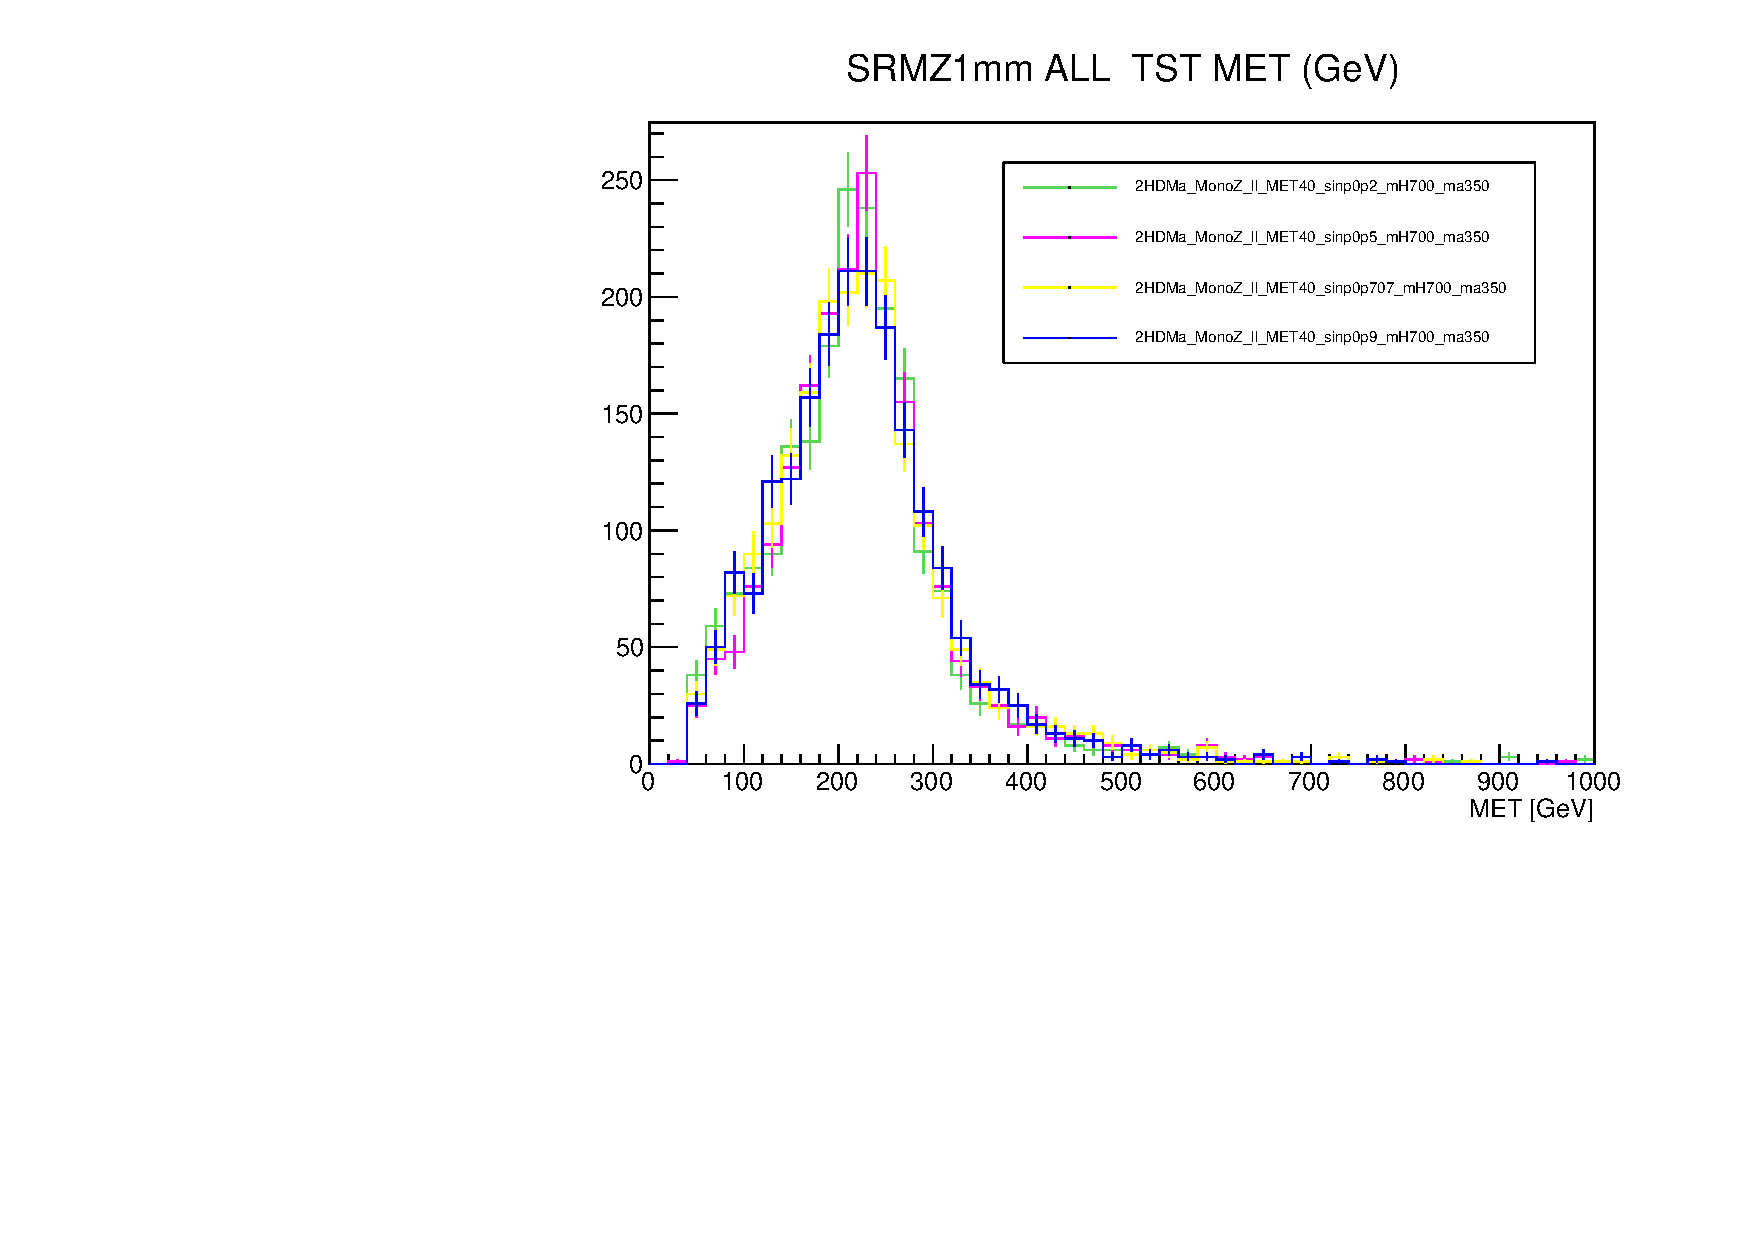
\includegraphics[width=0.45\textwidth]{texinputs/04_grid/figures/monoz/leptonic/SinThetaScan_mH700ma350_MET.pdf}
\caption{Performing one dimensional scans of $\tan{\beta}$ for fixed \mA =600 \GeV and \ma = 150 \GeV (left) and $\sin{\theta}$ for fixed \mA = 600 \GeV and \ma = 250 \GeV (right) shows these parameter have little impact on the event's kinematic distributions.  For small values of \tanb, there is a slight softening and broadening of the \MET distribution due to the increased contribution from the top box diagram.}
\label{fig:monoz_kin_tanb_sintheta}
\end{figure}


\begin{figure}
\centering
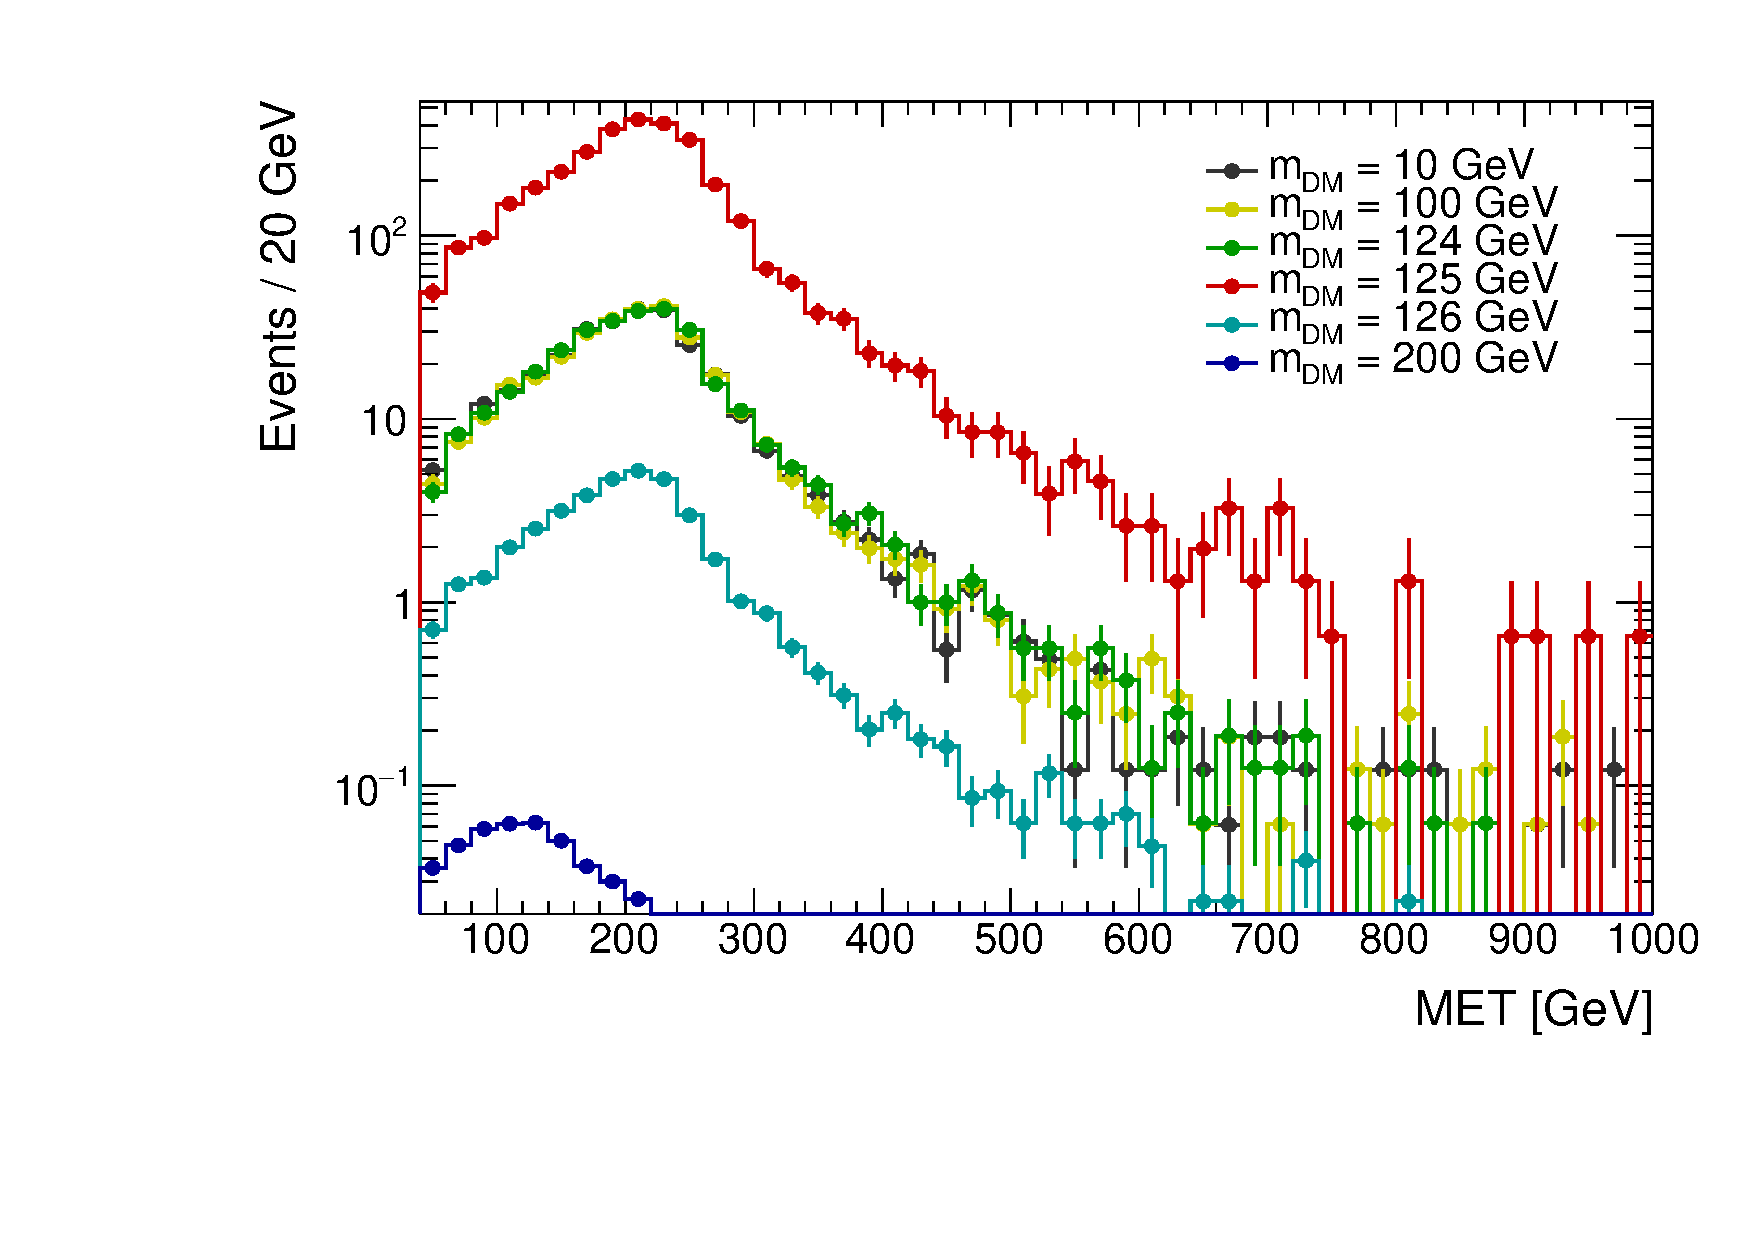
\includegraphics[width=0.6\textwidth]{texinputs/04_grid/figures/monoz/leptonic/dm_scan_met_ll.pdf}
\caption{In the DM mass scan, for $\mDM < \frac{\mH}{2}$, the DM mass has no effect on cross section or kinematic distributions, at $\mDM = \frac{\mH}{2}$ a resonant enhancement to the cross section occurs, and in the off-shell region where  $\mDM > \frac{\mH}{2}$ cross section steeply drops and the \MET distribution becomes more disperse.}
\label{fig:dm_scan_ll}
\end{figure}


\begin{figure}
\centering
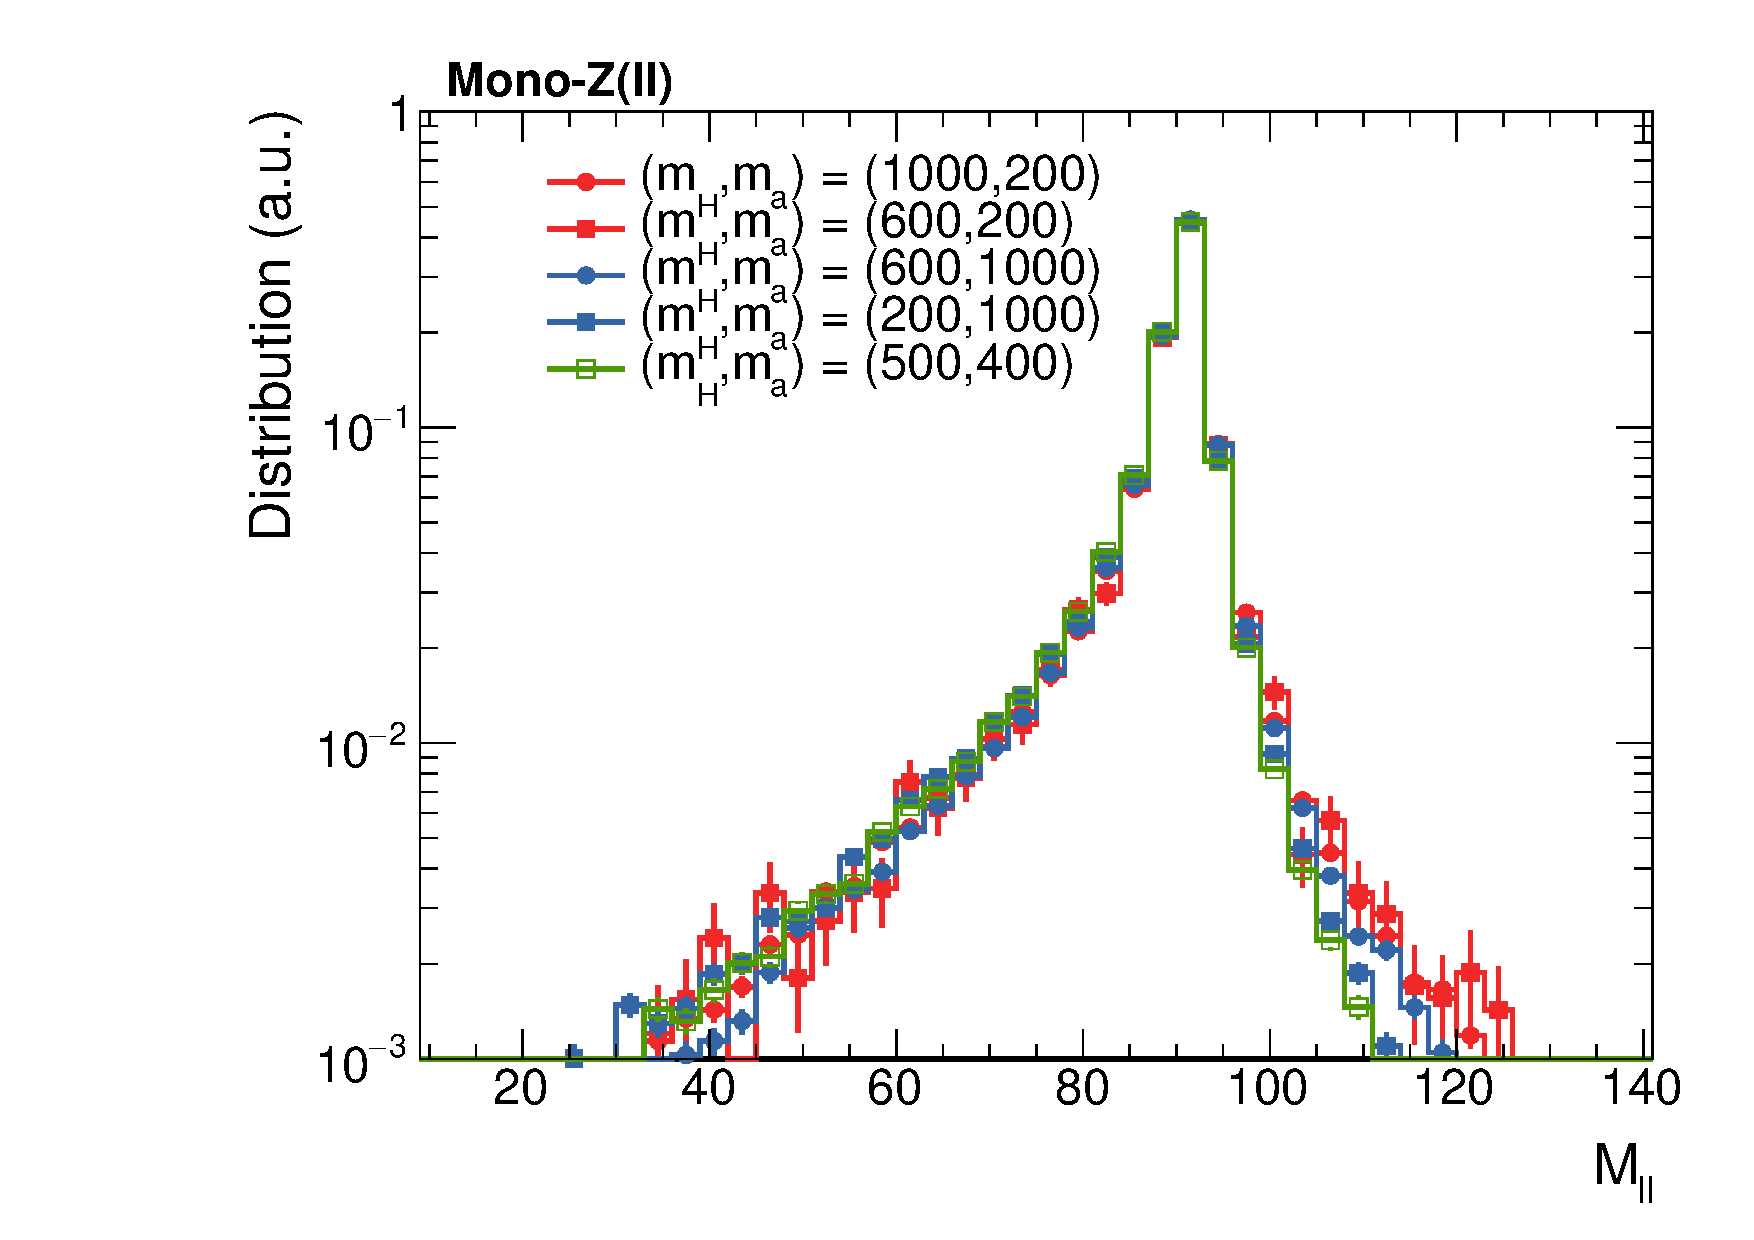
\includegraphics[width=0.45\textwidth]{texinputs/04_grid/figures/monoz/leptonic/inclusive_h_mz_lep.pdf}
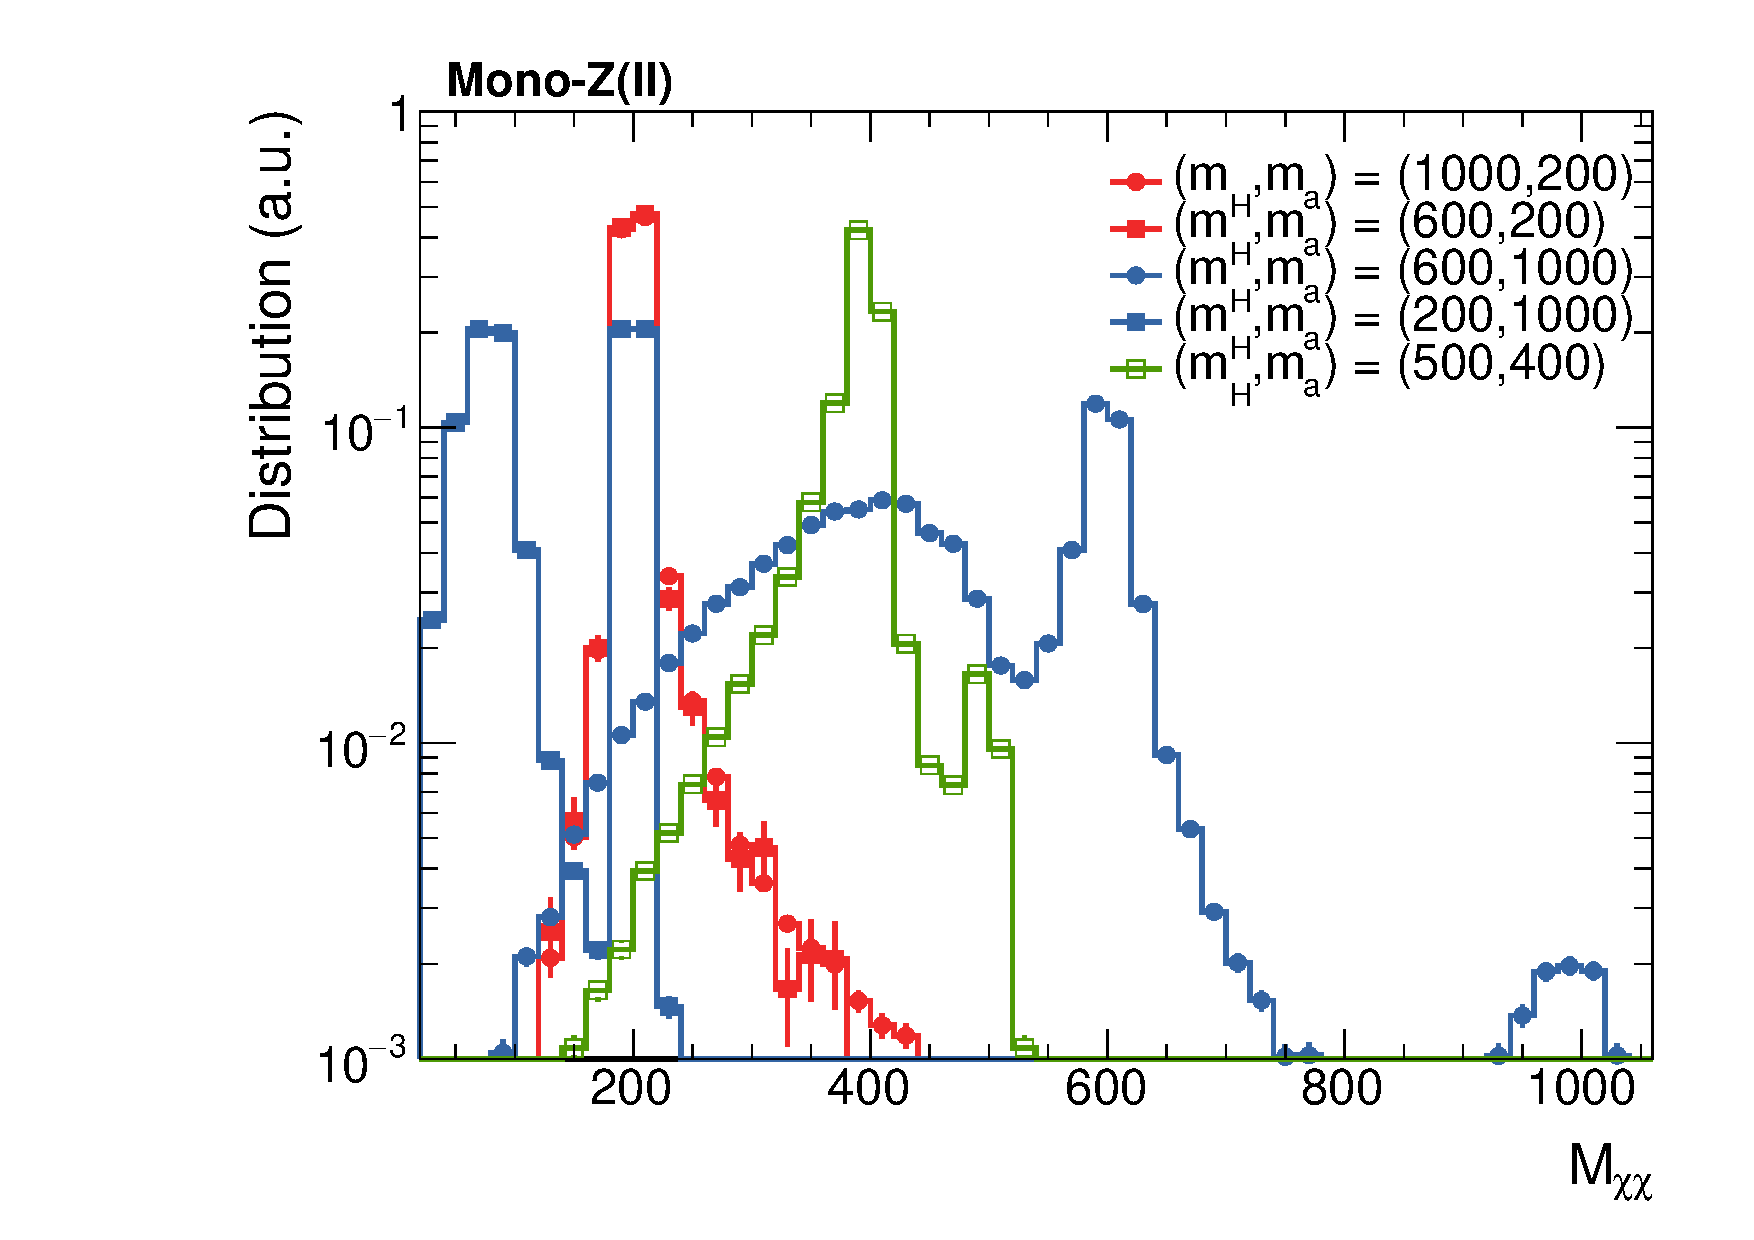
\includegraphics[width=0.45\textwidth]{texinputs/04_grid/figures/monoz/leptonic/inclusive_h_m_med_dm.pdf}
\caption{Distributions of the invariant mass of the dilepton (left) and $\chi\overline{\chi}$ systems (right) with no selection applied in addition to the generation cuts. The $M_{ll}$ distribution is centered around the Z boson mass independent of the chosen parameter point, indicating that there is no contribtion from $\gamma*$ exchange. The $M_{\chi\overline{\chi}}$ distribution }
\label{fig:monoz_kin_inclusive}
\end{figure}


\begin{figure}
\centering
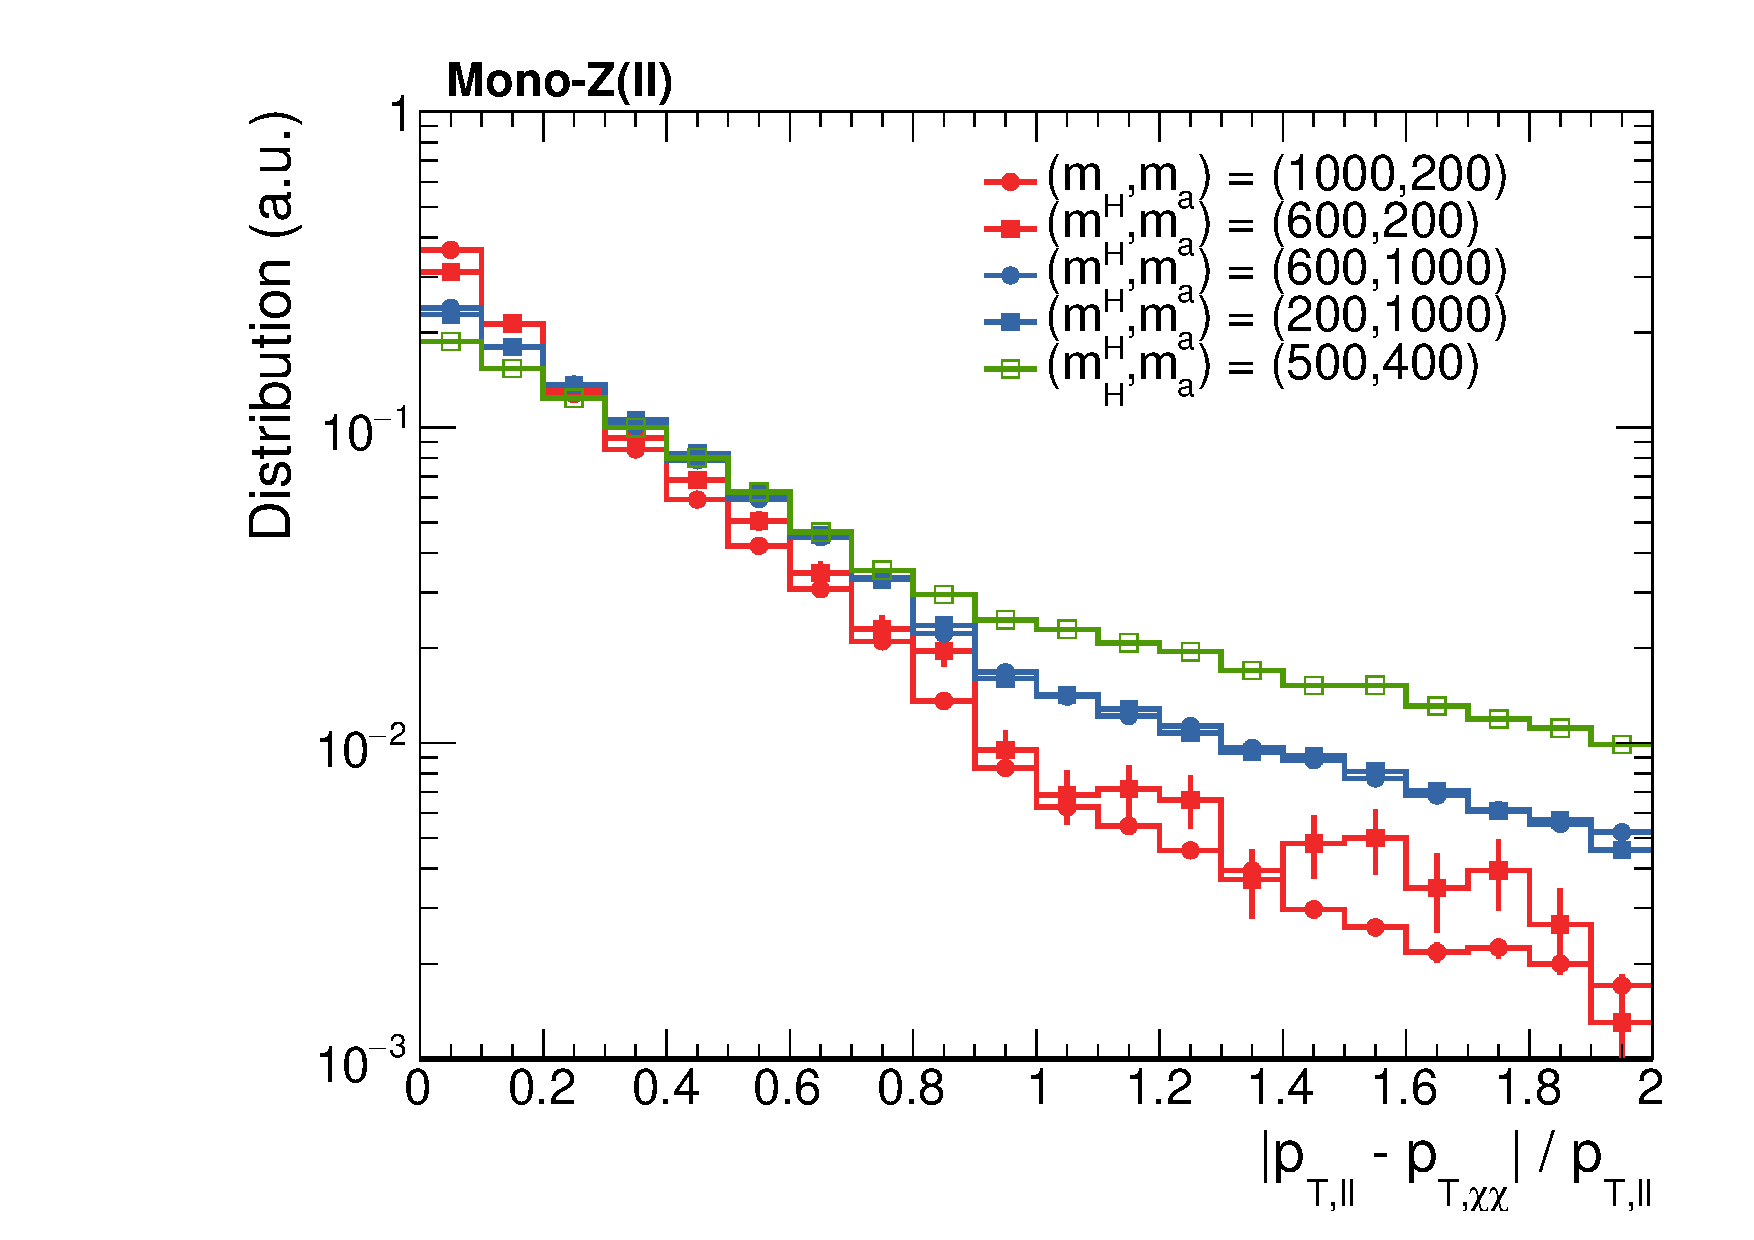
\includegraphics[width=0.45\textwidth]{texinputs/04_grid/figures/monoz/leptonic/presel_h_balance.pdf}
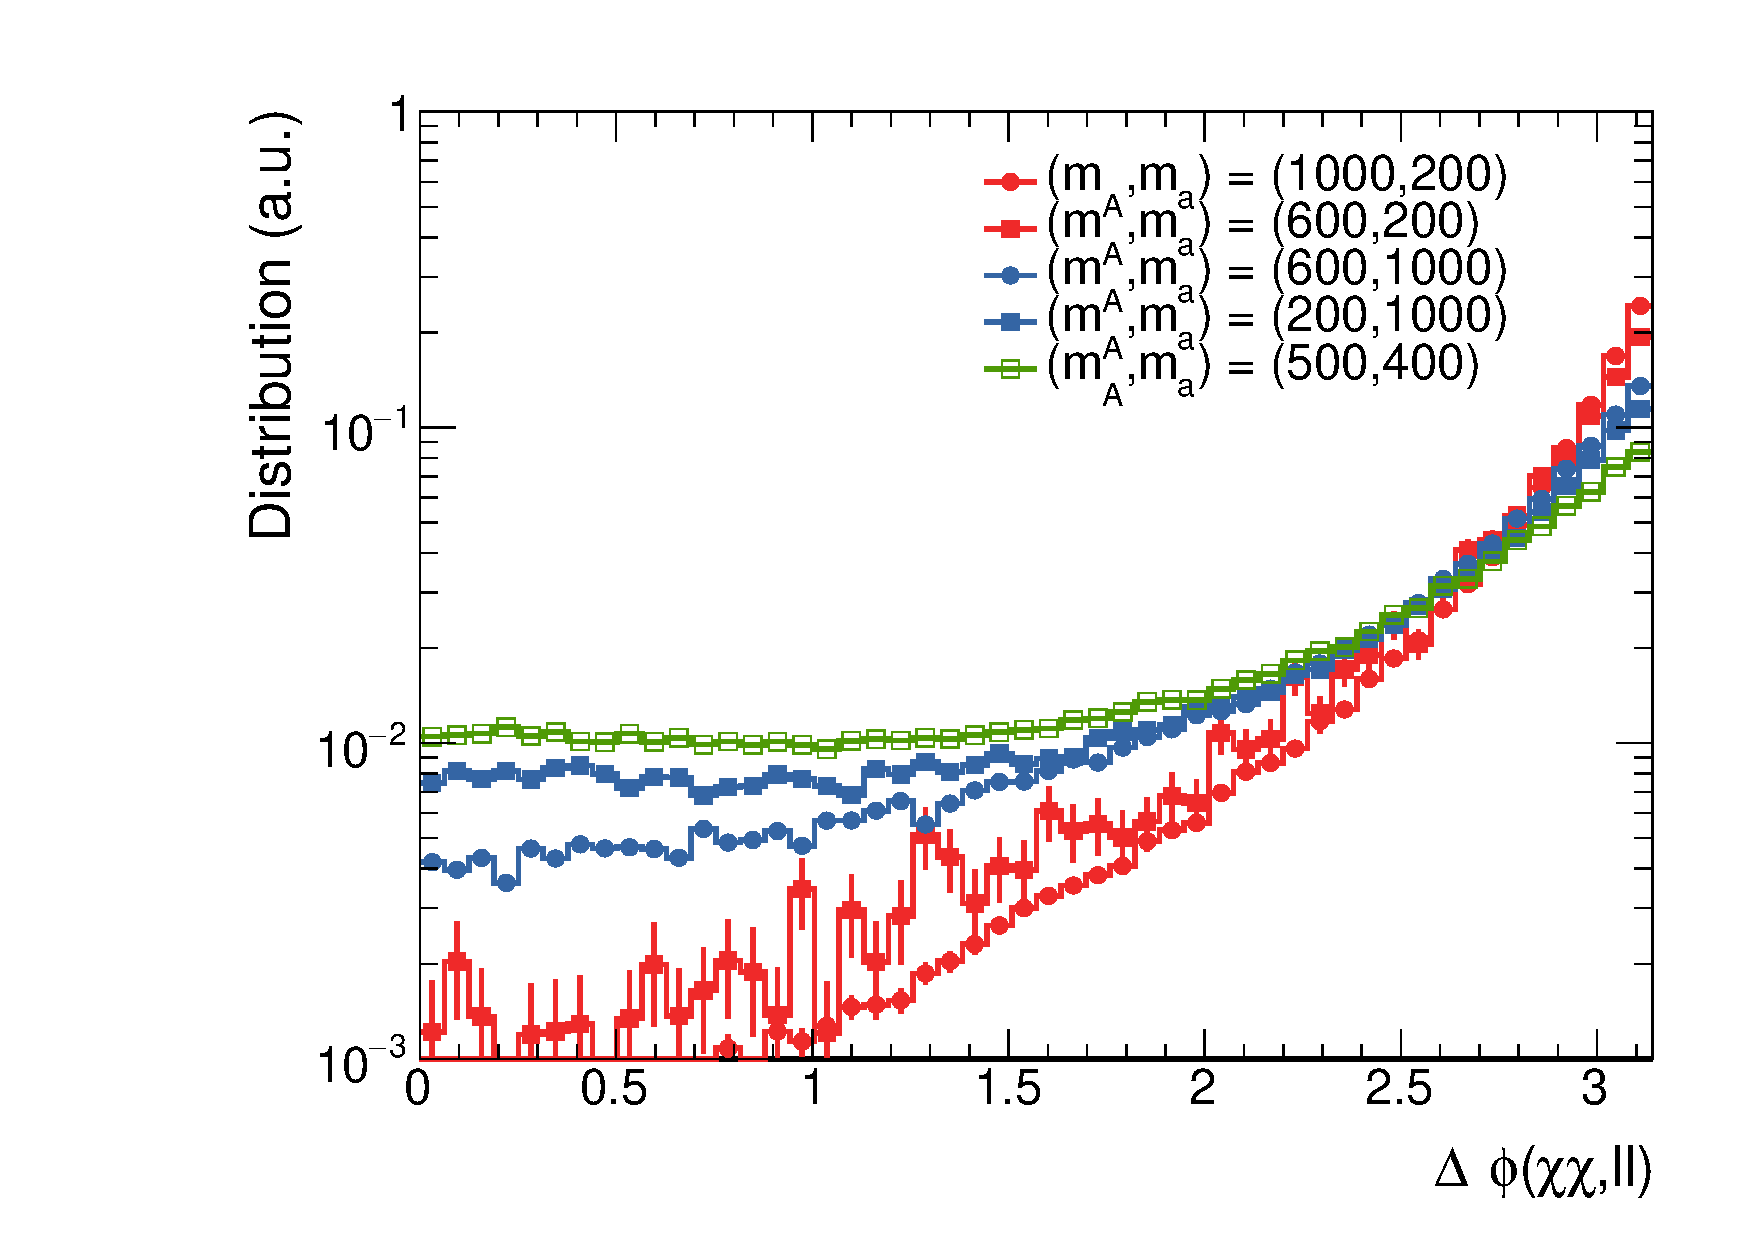
\includegraphics[width=0.45\textwidth]{texinputs/04_grid/figures/monoz/leptonic/presel_h_dphi_met_ll.pdf}
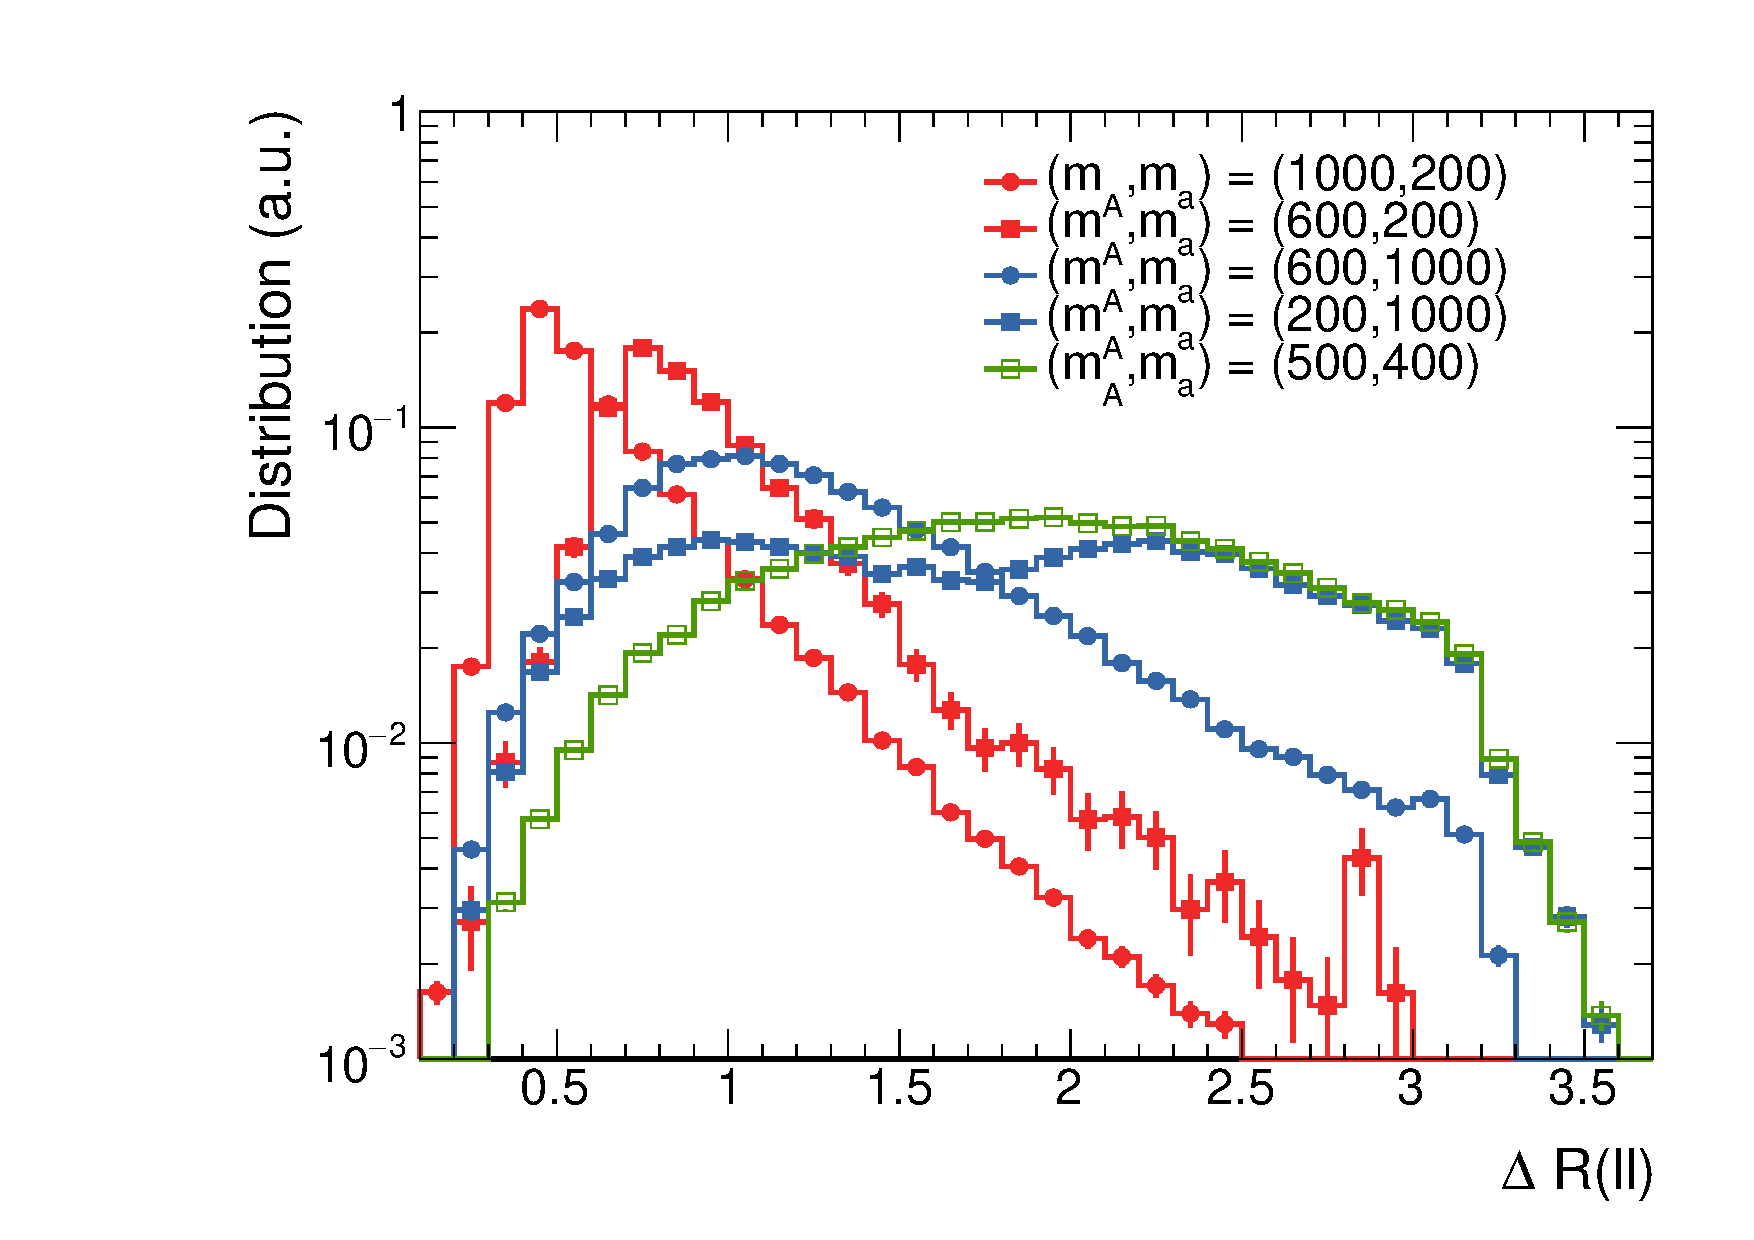
\includegraphics[width=0.45\textwidth]{texinputs/04_grid/figures/monoz/leptonic/presel_h_dr_ll.pdf}
\caption{Distributions of the main selection variables after preselection: \pt balance (top panel), $\Delta\Phi$ (middle) and $\Delta R$ (bottom). The shown parameter points illustrate the different qualitative behavior in the three different mass regions. }
\label{fig:monoz_kin_presel}
\end{figure}


\begin{figure}
\centering
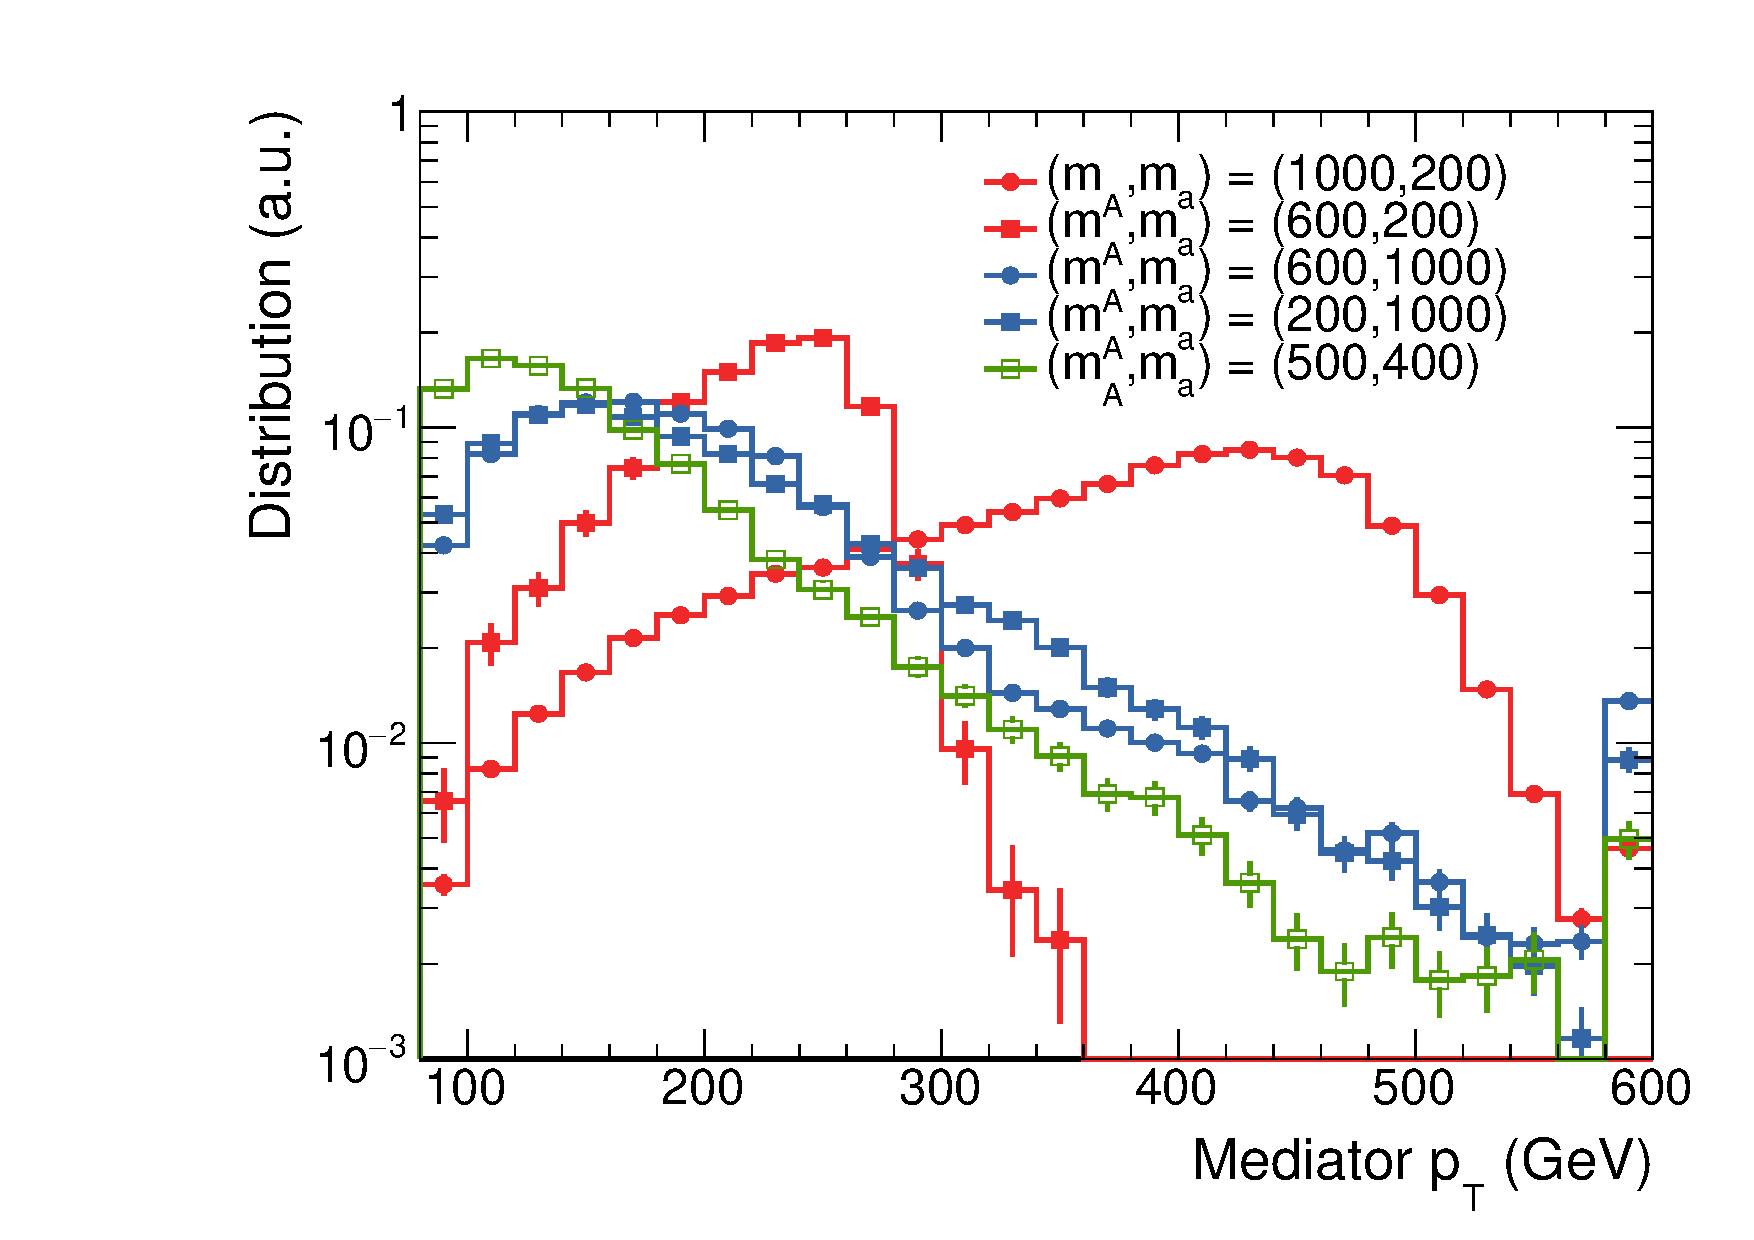
\includegraphics[width=0.45\textwidth]{texinputs/04_grid/figures/monoz/leptonic/dmwg-final_h_pt_med_dm.pdf}
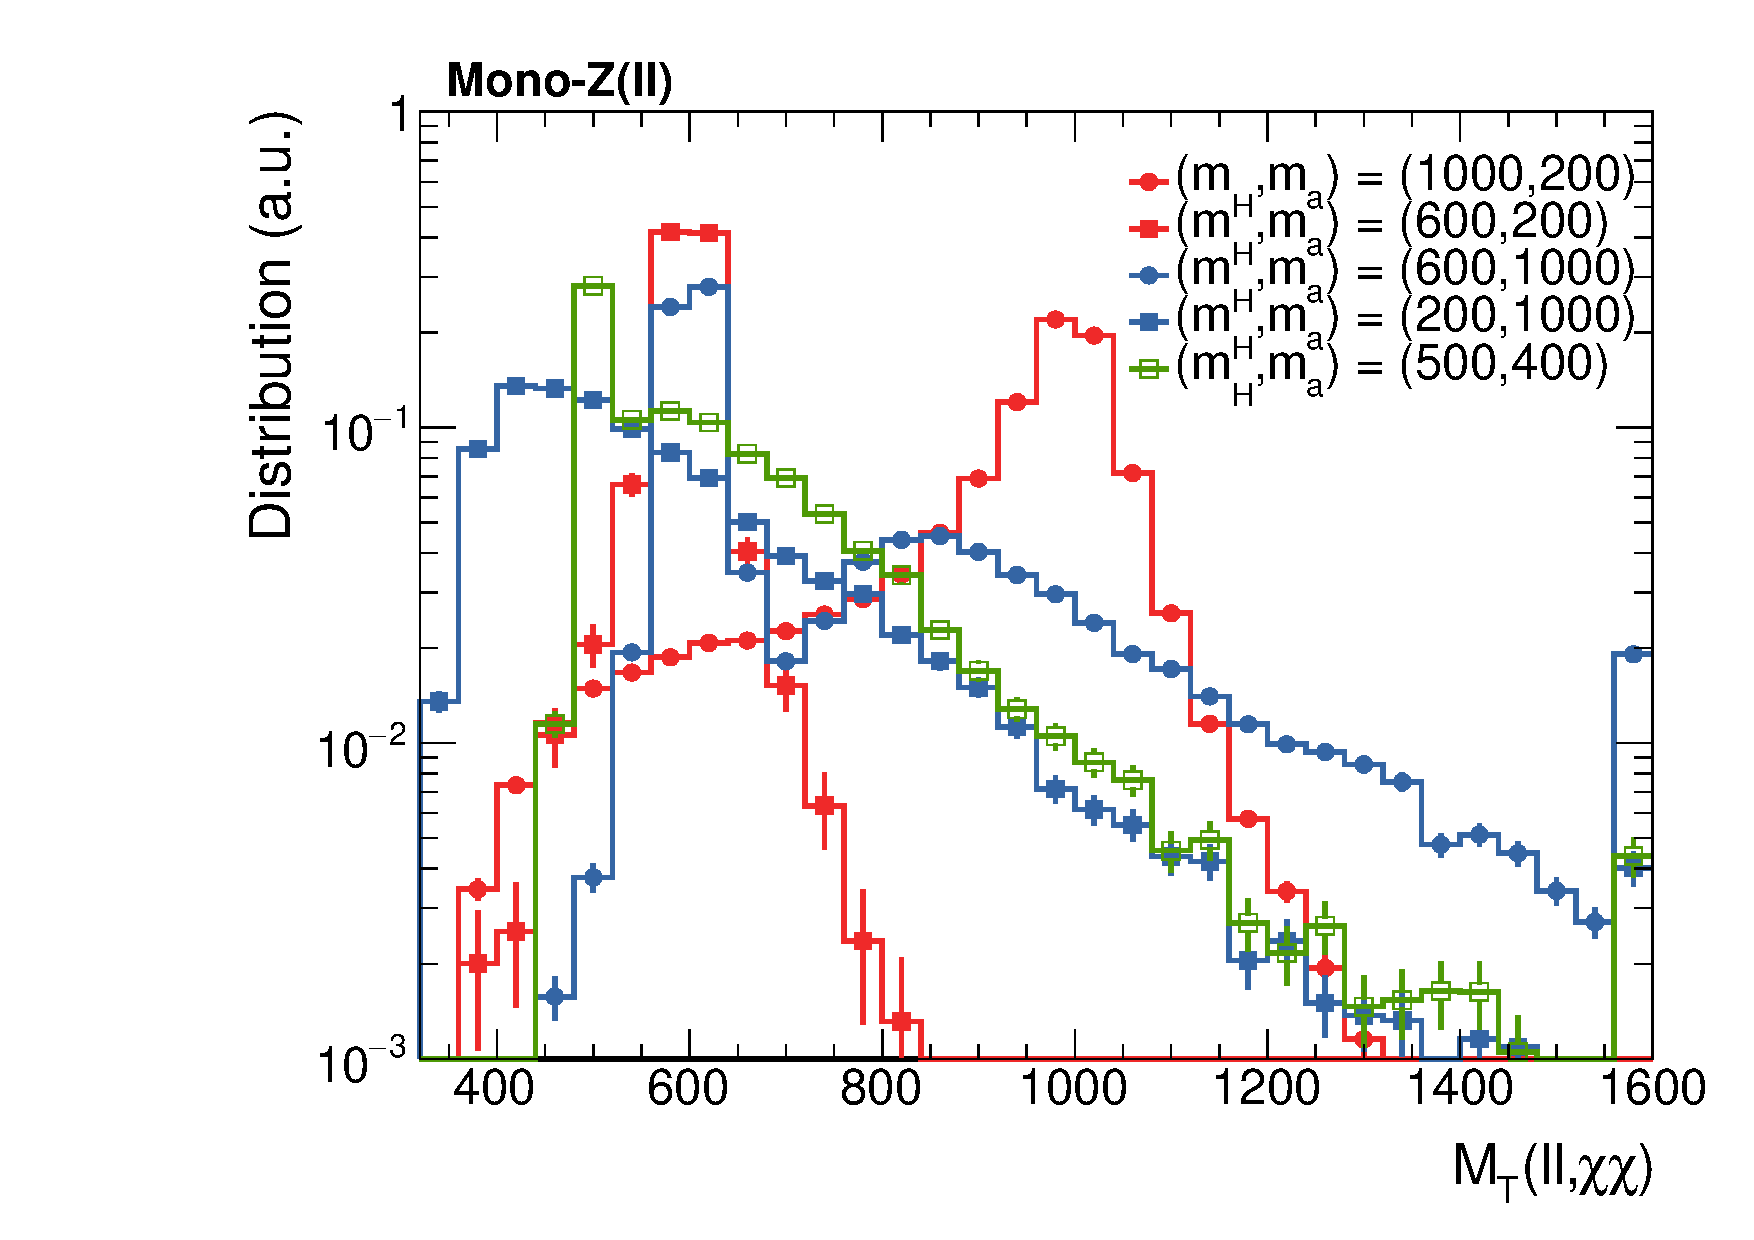
\includegraphics[width=0.45\textwidth]{texinputs/04_grid/figures/monoz/leptonic/dmwg-final_h_mt_total.pdf}
\caption{\MET and  MT distributions in the signal region. The \MET distribution shows a Jacobian structure in the $\mA > \ma$ regime, the location of which strongly depends on $\mA$. In the region of inverted mass hierarchy $\mA < \ma$, the spectrum is less structured and does not fall off as steeply towards higher values. For a small mass splitting of $\ma-\mA\approx M_{Z}$, the spectrum is shifted to much lower values of \MET. The MT distribution allows to access the resonant nature of the process. Clear mass peaks are present for the normal mass hierarchy. In the inverted region, the MT distribution is more sensitive to the mass difference $\ma-\mA$ than the \MET distribution, allowing to differentiate between signal hypotheses that give near-identical \MET distributions. }
\label{fig:monoz_kin_final}
\end{figure}


\begin{figure}
\centering
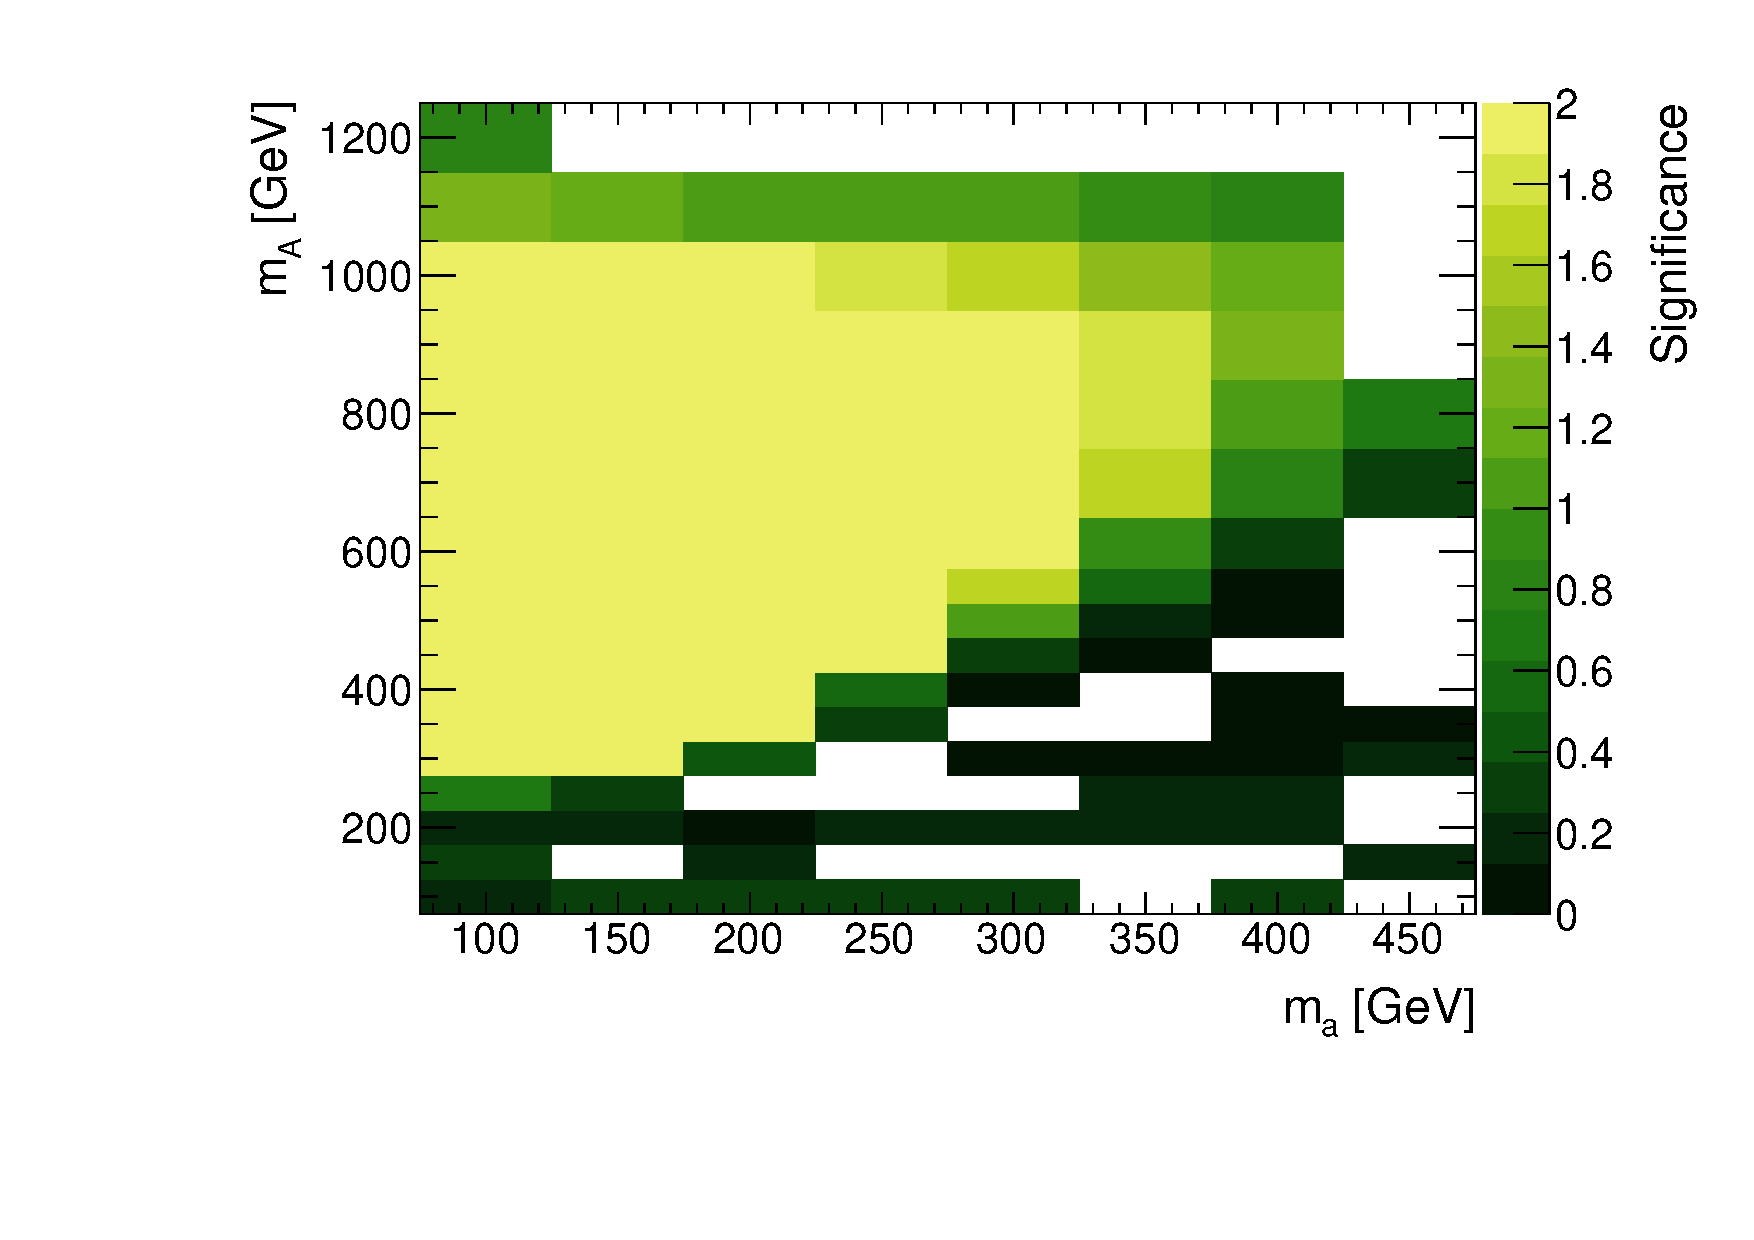
\includegraphics[width=0.9\textwidth]{texinputs/04_grid/figures/monoz/leptonic/mAma_Significance_ll.pdf}
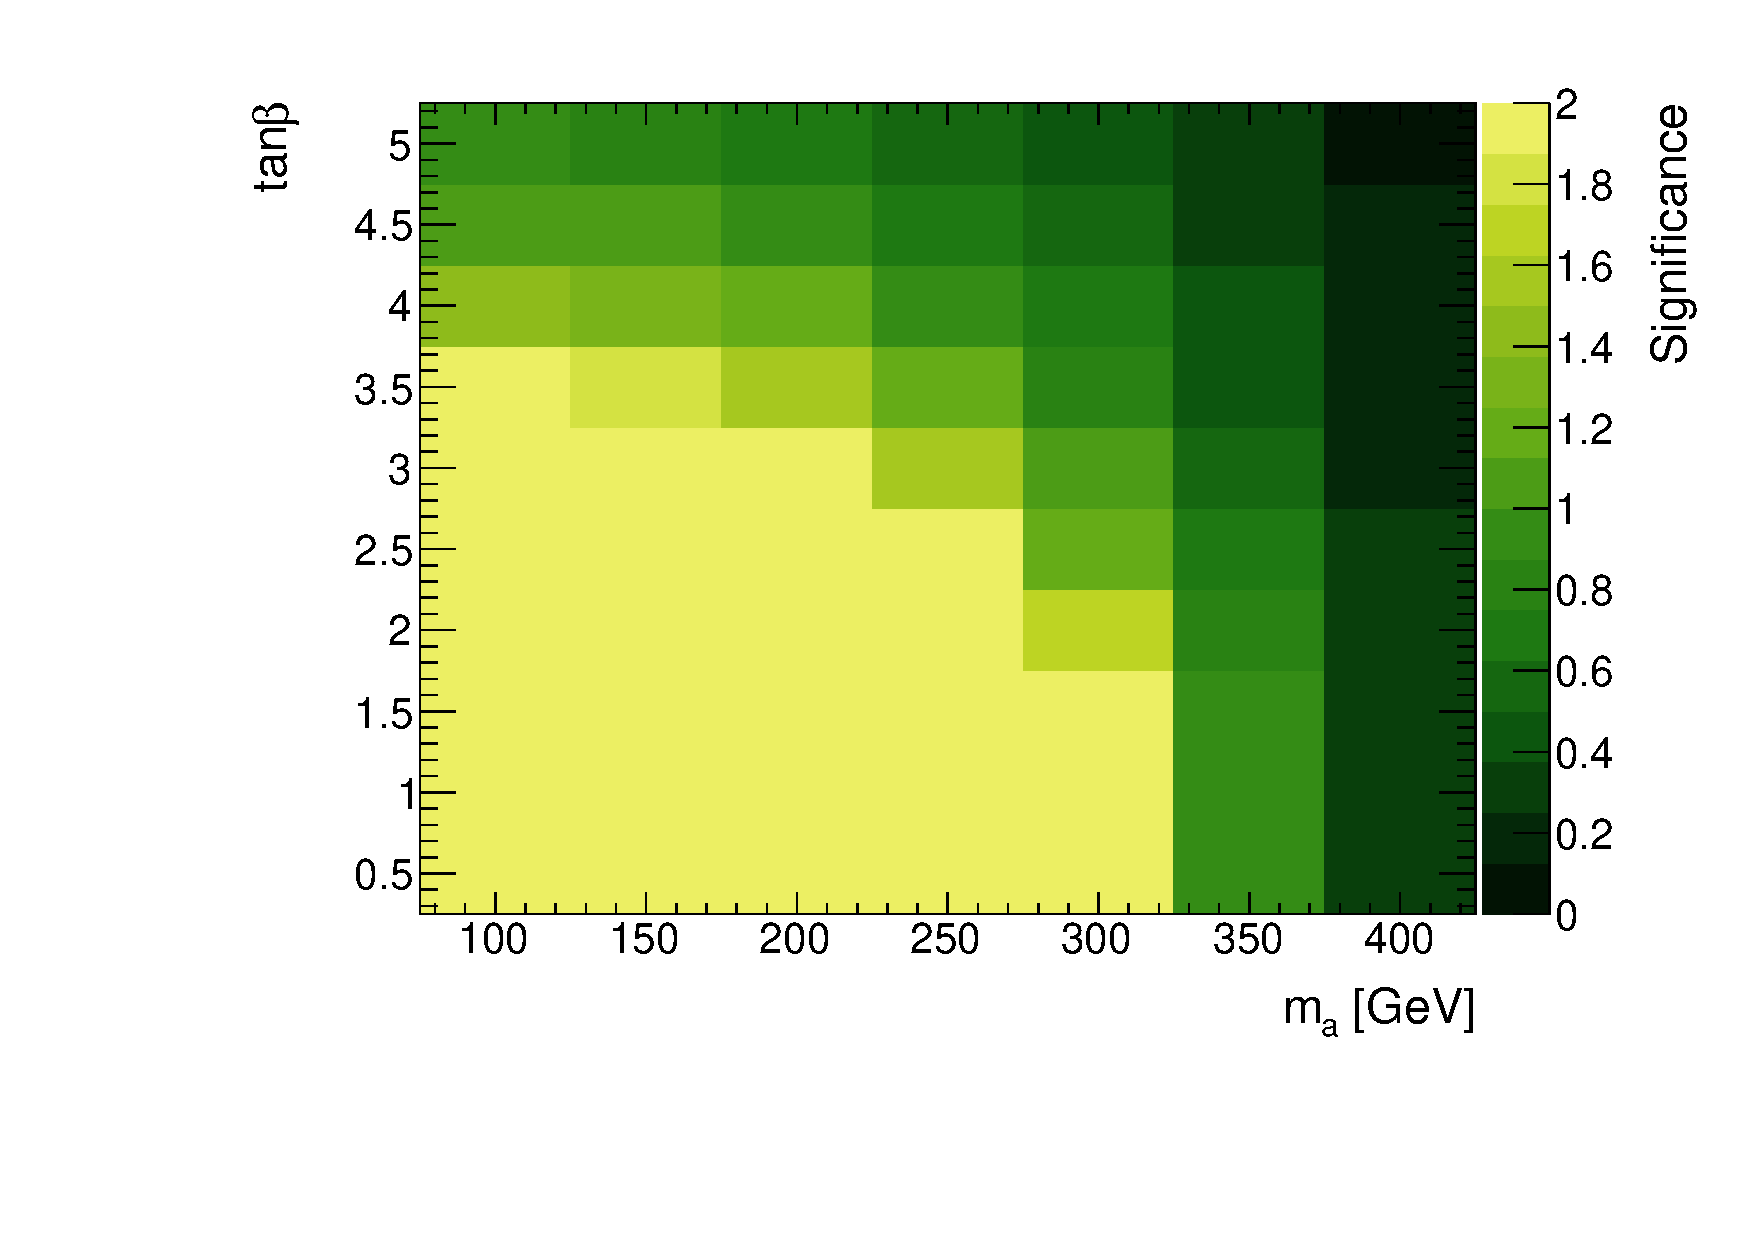
\includegraphics[width=0.9\textwidth]{texinputs/04_grid/figures/monoz/leptonic/tanbma_Significance_ll.pdf}
\caption{Expected significances are calculated using published background estimates and assuming a reconstruction efficiency of 75\%.  The ATLAS and CMS experiments are expected to be sensitive to regions with significances greater than 2.}
\label{fig:expected_significance_monozll}
\end{figure}

